%! Suppress = TooLargeSection
%! Suppress = SentenceEndWithCapital
%! Suppress = LineBreak
%! Suppress = MissingLabel
%! Suppress = Unicode
\documentclass[12pt]{article}
\usepackage{amsmath}
\usepackage{amsfonts}
\usepackage{graphicx}
\usepackage[colorinlistoftodos]{todonotes}
\usepackage[utf8]{inputenc}
\usepackage{lmodern}
\usepackage[MeX]{polski}
\usepackage{rotating}
\usepackage{geometry}
\usepackage{multirow}
\usepackage{xcolor,colortbl}
\usepackage{xparse}
\usepackage[most]{tcolorbox}
\usepackage{fancyvrb,newverbs,xcolor}
\usepackage{amssymb}
\usepackage{booktabs}
\usepackage{float}
\usepackage{minted}
\usepackage{multicol}
\usepackage{lineno}
\usepackage{hyperref}

\hypersetup{
    colorlinks=true,
    linkcolor=blue,
    filecolor=magenta,
    urlcolor=cyan,
}

\urlstyle{same}


\NewDocumentCommand{\newframedtheorem}{O{}momo}{%
\IfNoValueTF{#3}
{%
\IfNoValueTF{#5}
{\newtheorem{#2}{#4}}
{\newtheorem{#2}{#4}[#5]}%
}
{\newtheorem{#2}[#3]{#4}}
\tcolorboxenvironment{#2}{#1}%
}

\newframedtheorem{theorem}{Twierdzenie}[section]
\newframedtheorem{definition}[theorem]{Definicja}

\lstset{
  basicstyle=\ttfamily,
  mathescape
}


\renewcommand{\figurename}{Załącznik}

\begin{document}
    \begin{titlepage}

        \newcommand{\HRule}{\rule{\linewidth}{0.5mm}}

        \center

        \textsc{\LARGE Uniwerystet Jagielloński}\\[1.5cm]

        \HRule \\[0.4cm]
        %        { \huge \bfseries ETL}\\[0.4cm]
        \textsc{\Large Pytania do egzaminu licencjackiego}\\[0.5cm]
        \textsc{\large na kierunku Informatyka}\\[0.5cm]
        \HRule \\[1.0cm]

        \Large% \emph{Autorzy:}\\
        Małgorzata \textsc{Dymek}\\[1.5cm]

        
\includegraphics[scale=0.27]{uj.jpg}\\[4cm]

        {\large Rok akademicki 2019/2020}\\

        \vfill
    \end{titlepage}

    \tableofcontents

    \newpage


    \begin{center}{\LARGE Matematyczne podstawy informatyki}\end{center}

    \section{Zasada indukcji matematycznej.}

    \begin{theorem}
        \textbf{Zasada indukcji matematycznej.} Niech T(n) - funkcja/forma zdaniowana zmiennej $n \in \mathbb{N}$. Jeżeli:
        \begin{enumerate}
            \item zachodzi $T(0)$
            \item $\forall n \in \mathbb{N} ~~ T(n) \Rightarrow  T(n+1)$
        \end{enumerate}
        to wtedy $T(n)$ jest prawdziwa dla każdego $n \in \mathbb{N}$.
    \end{theorem}

    \textbf{Schemat dowodu:}\\

    Niech $M = \{ n \in \mathbb{N}: ~ T(n) ~ zachodzi \}$, $M \subset \mathbb{N}$. Wtedy wg twierdzenia:
    \begin{enumerate}
        \item $\Rightarrow 0 \in M$
        \item $\Rightarrow n \in M \Rightarrow n+1 \in M$
    \end{enumerate}
    Zatem z \textbf{aksjomatu 5} wnioskujemy M = N.

    \begin{theorem}
        \textbf{Aksjomat 5 liczb naturalnych (Peano)}. Niech będzie dany zbiór, którego elementami są liczby
        naturalne, o następujących właściwościach:
        \begin{enumerate}
            \item J jest elementem tego zbioru.
            \item Wraz z liczbą naturalną należącą do tego zbioru, należy do niego również jej następnik.
        \end{enumerate}
        Wtedy zbiór ten zawiera wszystkie liczby naturalne.
        $(Z \subset \mathbb{N}) \wedge (J \in Z) \wedge (\forall k \in \mathbb{N} k* \in Z) \Rightarrow Z = \mathbb{N}$.
    \end{theorem}

    Przykład: $2^1 + 2^2 + \cdots + 2^n = 2^{n+1} - 2$, Nierówność Bernoulliego
    $dla ~ h \geq -1 ~~ (1+h)^2 \geq 1 + n*h, ~~ \forall n \in \mathbb{N}^{+}$, $1 + 2 + \cdots + n = \frac{n(n+1)}{2} \forall n \in \mathbb{N}$

    \section{Porządki częściowe i liniowe. Elementy największe, najmniejsze, maksymalne i minimalne.}

    \begin{definition}
        \textbf{Częściowy porządek}. Niech X zbiór, $R \subset X \times X$ relacja. Wtedy R nazywamy \textbf{relacją częściowego porządku} w X
        $\Leftrightarrow$
        \begin{enumerate}
            \item R \textbf{zwrotna} ($\forall x \in X ~ xRx$),
            \item R \textbf{przechodnia} ($\forall x,y,z \in X ~ xRy \wedge yRz \Rightarrow xRz$),
            \item R \textbf{antysymetryczna} ($\forall x,y \in X ~ xRy \wedge yRx \Rightarrow x = y$).
        \end{enumerate}
        Piszemy: $\leqslant, \preceq, \prec gdy \neq$. \underline{Przykład:} $(\mathbb{R}, \leq)$, gdzie $x \preceq y \Leftrightarrow x \leq y ~ \forall x,y \in \mathbb{R}$.

        Wtedy $(\mathbb{R}, \preceq)$ jest cześciowym porządkiem.\\

        Jeżeli $(X, \mathbb{R})$ jest częściowym porządkiem, to elementy $x, y \in X$ nazywamy  \textbf{porównywalnymi}
        $\Leftrightarrow ~ xRy  \vee yRx$.\\

        \textbf{Diagram Hassego} - graf skierowany przedstawiający częściowy porządek w zbiorze, w odpowiedni sposób
        przedstawiony graficznie.
    \end{definition}

    \begin{definition}
        \textbf{Liniowy porządek}. Niech X zbiór, $R \subset X \times X$ relacja. Wtedy R nazywamy \textbf{relacją częściowego porządku} w X
        $\Leftrightarrow$
        \begin{enumerate}
            \item R \textbf{zwrotna} ($\forall x \in X ~ xRx$),
            \item R \textbf{przechodnia} ($\forall x,y,z \in X ~ xRy \wedge yRz \Rightarrow xRz$),
            \item R \textbf{antysymetryczna} ($\forall x,y \in X ~ xRy \wedge yRx \Rightarrow x = y$),
            \item R \textbf{spójna} ($\forall x,y \in X ~ xRy \vee yRx \vee x = y$).
        \end{enumerate}
    \end{definition}

    \begin{definition}
        Niech $\preceq$ jest relacją częściowego porządku wówczas element $m$ jest to:
        \begin{enumerate}
            \item \textbf{Element maksymalny}, jeśli $~~ \forall a \in A ~~ m \preceq a ~ \Rightarrow  ~ a = m$,
            \item \textbf{Element minimalny}, jeśli $~~ \forall a \in A ~~ a \preceq m ~ \Rightarrow  ~ a = m$,
            \item \textbf{Element największy}, jeśli $~~ \forall a \in A ~~ a \preceq m$,
            \item \textbf{Element najmniejszy}, jeśli $~~ \forall a \in A ~~ m \preceq a$.
        \end{enumerate}
    \end{definition}

    Przykłady - sprawdź czy porządek: $xRy \Leftrightarrow x | y$


    \newpage

    \section{Relacja równoważności i zbiór ilorazowy.}

    \begin{definition}
        Relację $R \subset X \times X$ nazywamy \textbf{relacją równoważości} $\Leftrightarrow$ relacja R jest:
        \begin{enumerate}
            \item \textbf{zwrotna} ($\forall x \in X ~ xRx $),
            \item \textbf{symetryczna} ($\forall x,y \in X ~ xRy \Rightarrow yRx$),
            \item \textbf{przechodnia} ($\forall x,y,z \in X ~ xRy \wedge yRz \Rightarrow xRz$).
        \end{enumerate}
    \end{definition}

    \begin{definition}
        Niech $R \subset X \times X$ będzie relacją równoważności, $X \neq \varnothing$, $x \in X$. \textbf{Klasą abstrakcji}
        elementu x (wzgledem relacji R) nazywamy:

        $[x]_{R} = {y \in X: xRy}$

        Element x nazywamy reprezentantem klasy abstrakcji $[x]_{R}$.
    \end{definition}

    \begin{definition}
        \textbf{Zbiorem ilorazowym} zbioru X przez relację R nazywamy zbiór wszystkich klas abstrakcji.

        $X/R = {[y]_{R}: x \in X} ~~ \subset X$
    \end{definition}

    Przykład: $xRy ~ \Leftrightarrow x \equiv_3 y$.

    \newpage


    \section{Metody dowodzenia twierdzeń: wprost, nie wprost, przez kontrapozycję.}

    Dla prawdziwości zdania:
    \begin{align*}
        p \Rightarrow q
    \end{align*}

    \begin{definition}
        \textbf{Dowód wprost}. Metoda dowodu wprost polega na założeniu, że p jest prawdą i pokazaniu, że wówczas q
        jest prawdą.
    \end{definition}

    \begin{definition}
        \textbf{Dowód nie wprost}. Metoda dowodu nie wprost opiera się na następującej tautologii rachunku
        zdań, zwanej prawem kontrapozycji:
        \begin{align*}
            (p \Rightarrow q) \Leftrightarrow (\neg q \Rightarrow \neg p).
        \end{align*}
        Zatem stosując tę metodę zakładamy, że q jest zdaniem fałszywym i pokazujemy, że p jest również
        zdaniem fałszywym.
    \end{definition}

    \begin{definition}
        \textbf{Dowód przez zaprzeczenie} Metoda dowodu przez zaprzeczenie opiera się na następującej tautologii rachunku
        zdań:
        \begin{align*}
            (p \Rightarrow q) ~ \Leftrightarrow ~ (\neg p \vee q) ~ \Leftrightarrow ~ \neg(p \wedge \neg q)
        \end{align*}
        Stosując to podejście zakładamy, że p jest prawdą a q fałszem i pokazujemy, że prowadzi to do sprzeczności,
        to znaczy, pokazujemy że $(p \wedge \neg q)$ jest fałszem.
    \end{definition}

    \newpage

    \section{Metody numeryczne rozwiązywania równań nieliniowych: bisekcji, siecznych, Newtona.}

    \subsection{Metoda połowienia (bisekcji)}

    \textbf{Założenia:}
    \begin{itemize}
        \item $f$ jest funkcją ciągłą w przedziale $[a,b]$,
        \item $f(a)f(b) < 0$.
    \end{itemize}
    Z własności Darboux funkcji ciągłych, funkcja f ma miejsce zerowe w przedziale $[a,b]$.

    \begin{definition}
        \textbf{Algorytm bisekcji} polega na obliczeniu $f(c_k)$, gdzie $c_k = \frac{a_k + b_k}{2}$ i zastąpieniu przez
        $c_k$ tej z liczb $a_k, b_k$ dla której funkcja $f$ ma taki sam znak.
        \begin{center}
            $(a_{k+1}, b_{k+1}) = (c_k, b_k)$ jeżeli $f(a_k)f(c_k) > 0$\\
            $(a_{k+1}, b_{k+1}) = (a_k, c_k)$ jeżeli $f(b_k)f(c_k) > 0$
        \end{center}
        Jeżeli $f(c_k) = 0$ to kończymy obliczenia.
    \end{definition}
    \begin{itemize}
        \item Metoda bisekcji jest \textbf{niezawodna}, ale \textbf{wolno zbieżna}.
        \item W każdym kroku szerokość przedziału jest dzielona przez dwa.
        \item Kryteria zakończednia obliczeń:
        \begin{itemize}
            \item osiągnięto dokładność $\delta: |e_n| < \delta$
            \item wartość funkcji jest bliska 0: $f(c_n) < \epsilon$
            \item wykonano M iteracji
        \end{itemize}
        \item Algorytm bisekcji w k-tej iteracji przybliża rozwiązanie $\alpha$ z \textbf{dokładnością:} $|x_k - \alpha| \leq \frac{|b - a|}{2^k}$.
    \end{itemize}


    \subsection{Metoda siecznych}

    \textbf{Założenia:}
    \begin{itemize}
        \item $f$ jest funkcją ciągłą w przedziale $[a,b]$,
        \item $f(a)f(b) < 0$.
    \end{itemize}

    \begin{align*}
        x_{k+1} = x_k - \frac{f(x_k)(x_k - x_{k-1})}{f(x_k) - f(x_{k-1})}
    \end{align*}
    gdzie $x_0 = a$, $x_1 = b$.

    \begin{itemize}
        \item W metodzie siecznych rezygnujemy z założenia, że funkcja na końcach przedziału ma rózne znaki.
        \item Należy kontrolować zachowanie otrzymanego ciągu. \textbf{Może się zdarzyć, że metoda wyprodukuje ciąg rozbieżny!}
        \item korzyćci płynące ze stosowania tej metody to zdecydowanie \textbf{szybsza zbieżność} ciągu iteracji, jeśli
        $x_n, x_{n+1}$ juz są dobrymi \textbf{przybliżeniami pierwiastka}.
    \end{itemize}

    \subsection{Metoda Newtona (stycznych)}

    \begin{align*}
        x_{n+1} = x_n - \frac{f(x_n)}{f'(x_n)}
    \end{align*}

    \textbf{Zmodyfikowana metoda Newtona:}
    \begin{align*}
        x_{n+1} = x_n - \frac{f'(x_n) \pm \sqrt{(f'(x_n))^2 - 2f(x_n)f''(x_n)}}{f''(x_n)}
    \end{align*}


    \begin{itemize}
        \item Metoda Newtona w wielu sytuacjach daje \textbf{bardzo szybką zbieżność}.
        \item Podstawową wadą tej metody jest konieczność obliczenia pochodnej funkcji.
        \item Zmodyfikowana metoda Newtona daje bardzo szybką zbieżność, jeśli $x_n$ jest już dobrym przybliżeniem
        pierwiastka.
        \item Koszt wyznaczenia kolejnego przybliżenia w zmodyfikowanej metodzie może przerastać korzyści płynące
        z szybszej zbieżności.
    \end{itemize}

    \textbf{Wielowymiarowa metoda Newtona}.\\

    Jeśli $f = (f_1, f_2, \dots, f_n): \mathbb{R}^n \rightarrow \mathbb{R}^n$ jest różniczkowalną funkcją wielu zmiennych
    możemy przybliżyć ją lokalnie:

    \begin{align*}
        f(x) \approx f(x_0) + Df(x_0)(x - x_0)
    \end{align*}

    gdzie

    \begin{align*}
        Df(x_0) =
        \begin{bmatrix}
            \frac{\delta f_1}{\delta x_1}(x_0) & \frac{\delta f_1}{\delta x_2}(x_0) & \dots & \frac{\delta f_1}{\delta x_n}(x_0)\\
            \frac{\delta f_2}{\delta x_1}(x_0) & \frac{\delta f_2}{\delta x_2}(x_0) & \dots & \frac{\delta f_2}{\delta x_n}(x_0)\\
            \dots & \dots & \dots & \dots\\
            \frac{\delta f_n}{\delta x_1}(x_0) & \frac{\delta f_n}{\delta x2}(x_0) & \dots & \frac{\delta f_n}{\delta x_n}(x_0)
        \end{bmatrix}
    \end{align*}

    Rozwiązując równanie $f(x_0) + Df(x_0)(x - x_0) = 0$ otrzymujemy:
    \begin{align*}
        x^{(i+1)} = x^{(i)} - [Df(x^{(i)})]^{-1} f(x^{(i)})
    \end{align*}
    \begin{align*}
    [Df(x^{(i)})]
        ( x^{(i+1)} - x^{(i)} ) = -f(x^{(i)})
    \end{align*}

    \newpage

    \section{Rozwiązywanie układów równań liniowych: metoda eliminacji Gaussa, metody iteracyjne Jacobiego i Gaussa-Seidla.}

    \subsection{Metoda eliminacji Gaussa}

    Obliczając rząd macierzy metodą Gaussa należy za pomocą operacji elementarnych na wierszach sprowadzić macierz do
    macierzy schodkowej. Wtedy wszystkie niezerowe wiersze są liniowo niezależne i można łatwo odczytać rząd macierzy.

    \begin{align*}
        \begin{bmatrix}
            1 & -1 & 2 & 2\\
            2 & -2 & 1 & 0\\
            -1 & 2 & 1 & -2\\
            2 & -1 & 4 & 0
        \end{bmatrix}
        \stackrel{w_2 - 2w_1, w_3 + w_1, w_4 - 2w_1}{\sim}
        \begin{bmatrix}
            1 & -1 & 2 & 2\\
            0 & 0 & -3 & -4\\
            0 & 1 & 3 & 0\\
            0 & 1 & 0 & -4
        \end{bmatrix}
        \stackrel{w_2 \leftrightarrow w_3}{\sim}
        \begin{bmatrix}
            1 & -1 & 2 & 2\\
            0 & 1 & 3 & 0\\
            0 & 0 & -3 & -4\\
            0 & 1 & 0 & -4
        \end{bmatrix}
        \sim
    \end{align*}

    \begin{align*}
        \stackrel{w4 - w_2}{\sim}
        \begin{bmatrix}
            1 & -1 & 2 & 2\\
            0 & 1 & 3 & 0\\
            0 & 0 & -3 & -4\\
            0 & 0 & -3 & -4
        \end{bmatrix}
        \stackrel{w4 - w_3}{\sim}
        \begin{bmatrix}
            1 & -1 & 2 & 2\\
            0 & 1 & 3 & 0\\
            0 & 0 & -3 & -4\\
            0 & 0 & 0 & 0
        \end{bmatrix}
    \end{align*}

    \hfill \\
    \begin{center}{\large Metody iteracyjne}\end{center}
    Ogólna postać metody iteracyjnej:
    \begin{align*}
        Ax = b
    \end{align*}
    \begin{align*}
        Qx^{n+1} = (Q - A)x^n + b = \tilde{b}
    \end{align*}

    \begin{align*}
        x^0 = (0,0,0)
    \end{align*}
    \begin{align*}
        \begin{bmatrix}
            5 & -2 & 3\\
            2 & 4 & 2\\
            2 & -1 & -4\\
        \end{bmatrix}
        \begin{bmatrix}
            x_1\\
            x_2\\
            x_3\\
        \end{bmatrix}
        =
        \begin{bmatrix}
            10\\
            0\\
            0\\
        \end{bmatrix}
    \end{align*}
    \begin{align*}
        \left\{\begin{matrix}
                   5x_1 + (-2)x_2 + 3x_3 = 10\\
                   2x_1 + 4x_2 + 2x_3 = 0\\
                   2x_1 + (-1)x_2 + (-4)x_3 = 0\\
        \end{matrix}\right.
    \end{align*}

    \subsection{Metoda iteracyjna Jacobiego}

    \subsubsection{Algebraicznie}
    \begin{align*}
        \left\{\begin{matrix}
                   x^{N+1}_1 = \frac{1}{5}(10 + 2x^N_2 - 3x^N_3)\\
                   x^{N+1}_2 = \frac{1}{4}(-2x^N_1 - 2x^N_3)\\
                   x^{N+1}_3 = -\frac{1}{4}(x^N_2 - 2x^N_1)
        \end{matrix}\right.
    \end{align*}

    \subsubsection{Macierzowo}
    \begin{align*}
        Q = D ~~ \text{(diagonalna)}
    \end{align*}

    \subsection{Metoda iteracyjna Gaussa-Seidla}
    \subsubsection{Algebraicznie}
    \begin{align*}
        \left\{\begin{matrix}
                   x^{N+1}_1 = \frac{1}{5}(10 + 2x^N_2 - 3x^N_3)\\
                   x^{N+1}_2 = \frac{1}{4}(-2x^N_1 - 2x^{N+1}_3)\\
                   x^{N+1}_3 = -\frac{1}{4}(x^{N+1}_2 - 2x^{N+1}_1)
        \end{matrix}\right.
    \end{align*}

    \subsubsection{Macierzowo}
    \begin{align*}
        Q = L + D ~~ \text{(diagonalna i dolnotrójkątna)}
    \end{align*}


    \newpage

    \section{Wartości i wektory własne macierzy: numeryczne algorytmy ich wyznaczania.}
    \begin{align*}
        A \in \mathbb{C}^{n \times n} ~~~ \text{szukamy} ~~~ \lambda \in \mathbb{C}
    \end{align*}
    \begin{definition}
        Jeżeli
        \begin{align*}
            Ax = \lambda x
        \end{align*}
        dla $x \neq 0$ to $\lambda$ jest \textbf{wartością własną} A, a x - \textbf{wektorem własnym}
        A odpowiadającym $\lambda$.
    \end{definition}

    \subsection{Metoda potęgowa}
    \begin{align*}
        Ax = \lambda x\\
        x^{N+1} = A^{N+1} x^0\\
    \end{align*}

    \newpage

    \section{Interpolacja wielomianowa: metody Lagrange'a i Hermite'a. Efekt Rungego.}

    \subsection{Interpolacja wielomianowa}

    Interpolacja wielomianowa jest metodą numeryczną przybliżania funkcji.
    Wielomian p o możłiwie najniższym stopniu interpoluje wartości $y_k$ w węzłąch $x_k$ gdy dla danych $n+1$ punktów $(x_i, y_i)$
    \begin{align*}
        p(x_i)=y_i  \quad (0\leq i \leq n)
    \end{align*}
    Jeśli są to wartości pewnej funkcji $f$ to mówimy też że $p$ interpoluje $f$.

    \subsection{Wzór interpolacyjny Lagrange'a}

    Wyrażamy wielomian $p$ jako sumę
    \begin{align*}
        p(x)=\sum _{k=0}^{n}y_{i}l_k(x)
    \end{align*}
    w której $l_k$ są wielomianami zależnymi od węzłów $x_0,x_1, \dots x_n$ ale nie od wartości $y_0,y_1, \dots ,y_n$. Gdyby jedna z nich, mianowicie $y_i$, była równa 1, a pozostałe by znikały, to mielibyśmy równość
    \begin{align*}
        \delta_{ij} = p_n(x_j)=\sum _{k=0}^{n}y_{i}l_k(x_j)=\sum _{k=0}^{n}\delta_k l_k (x_j)=l_i(x_j) \quad (0 \leq j \leq n)
    \end{align*}

    ($\delta_ij$ jest deltą Kroneckera). Łatwo znaleźć wielomian $l_i$ o tej własności. Jego zerami są wszystkie węzły oprócz $x_i$, czyli dla pewniej stałej c jest
    \begin{align*}
        l_i(x)=c(x-x_0)\dots(x-x_{i-1})(x-x_{i+1})\dots(x-x_n)
    \end{align*}
    a $c$ wynika z warunku $l_i(x_i)=1$:
    \begin{align*}
        l_i(x)=\prod _{j=0\land j\neq i}^{n}{\frac {x-x_{j}}{x_{i}-x_{j}}}. \quad (0 \leq i \leq n).
    \end{align*}

    Zatem wzór interpolacyjny Lagrange'a ma postać:

    \begin{align*}
        w(x)=\sum _{i=0}^{n}y_{i}\prod _{j=0\land j\neq i}^{n}{\frac {x-x_{j}}{x_{i}-x_{j}}}.
    \end{align*}

    \subsection{Interpolacja Hermite’a}

    Interpolacja umożliwiająca znalezienie wielomianu przybliżającego według wartości
    \begin{align*}
        y_{1}=f(x_{1}),y_{2}=f(x_{2}),\dots ,y_{n}=f(x_{n})
    \end{align*}
    na $n$ zadanych węzłach $x_{1},x_{2},\dots ,x_{n}$ oraz na wartościach pochodnych na wybranych węzłach

    \begin{align*}
        f'(x_{1}),f''(x_{1}),\dots ,f^{(k_{1})}(x_{1}),\dots ,f'(x_{n}),\dots ,f^{(k_{n})}(x_{n}).
    \end{align*}

    Węzeł zadany bez pochodnej jest węzłem pojedynczym, a węzeł z zadanymi pochodnymi $1,2,\dots ,k$ jest węzłem $k+1$-krotnym.

    \subsubsection{Algorytm}

    Algorytm jest podobny jak przy interpolacji Newtona. Kolumnę wypełnia się wszystkimi wartościami węzłów (jeżeli węzeł jest $k$-krotny, to umieszczamy go w tabeli $k$ razy)\\\\
    \begin{tabular}{|l|l|}
        \hline
        $x_i$    & $f(x_i)$ \\ \hline
        $x_0$    & $f(x_0)$ \\ \hline
        $x_1$    & $f(x_1)$ \\ \hline
        $x_2$    & $f(x_2)$ \\ \hline
        $\vdots$ & $\ddots$ \\ \hline
        $x_n$    & $f(x_n)$ \\ \hline
    \end{tabular}
    \\\\

    Następnie dopisuje się do każdej kolumny kolejne różnice dzielone, z tym wyjątkiem, że przy węzłach $k$-krotnych, $k>1$, gdzie, de facto, nie można obliczyć różnicy dzielonej, podstawia się wartości kolejnych pochodnych na węzłach podzielone przez silnię z liczby tych samych węzłów. (W tabeli przedstawiony jest $3$-krotny węzeł $x_{1}$).\\\\


    \begin{tabular}{|c|c|cc}
        \hline
        $x_i$ & $f(x_i)$ & \multicolumn{1}{c|}{$f[x_{i-1}]$}     & \multicolumn{1}{c|}{$f[x_{i-2},x_{i-1},x_i]$} \\ \hline
        $x_0$  & $f(x_0)$ & &                                            \\ \cline{1-3}
        $x_1$  & $f(x_1)$ & \multicolumn{1}{c|}{$f[x_0,x_1]$} &                                            \\ \hline
        $x_1$  & $f(x_1)$ & \multicolumn{1}{c|}{$f'(x_1)$}    & \multicolumn{1}{c|}{$f[x_0,x_1,x_1]$}      \\ \hline
        $x_1$  & $f(x_1)$ & \multicolumn{1}{c|}{$f'(x_1)$}    & \multicolumn{1}{c|}{$\frac{f''(x_1)}{2!}$} \\ \hline
        $x_2$  & $f(x_2)$ & \multicolumn{1}{c|}{$f[x_1,x_2]$} & \multicolumn{1}{c|}{$f[x_1,x_1,x_2]$}      \\ \hline
        $\vdots$ & $\vdots$   & \multicolumn{1}{c|}{$\vdots$}       &                                            \\ \hline
        $x_n$ & $f(x_n)$ & \multicolumn{1}{c|}{$f[x_{n-1},x_n]$} & \multicolumn{1}{c|}{$f[x_{n-2},x_{n-1},x_n]$} \\ \hline
    \end{tabular}\\\\

    Tabelę uzupełnia się do końca jak przy interpolacji Newtona, uznając ciągłe pochodne na węzłach wielokrotnych jako różnice dzielone rzędu drugiego.\\\\

    \begin{tabular}{|c|c|cccll}
        \hline
        $x_i$ &
        $f(x_i)$ &
        \multicolumn{1}{c|}{$f[x_{i-1}]$} &
        \multicolumn{1}{c|}{$f[x_{i-2},x_{i-1},x_i]$} &
        \multicolumn{1}{c|}{$f[x_{i-3},x_{i-2},x_{i-1},x_i]$} &
        \multicolumn{1}{c|}{$\dots$} &
        \multicolumn{1}{c|}{$f[x_{i-n},\dots,x_i]$} \\ \hline
        $x_0$ &
        $f(x_0)$ &
        &
        &
        \multicolumn{1}{l}{} &
        &
        \\ \cline{1-3}
        $x_1$ &
        $f(x_1)$ &
        \multicolumn{1}{c|}{$f[x_0,x_1]$} &
        &
        \multicolumn{1}{l}{} &
        &
        \\ \cline{1-4}
        $x_1$ &
        $f(x_1)$ &
        \multicolumn{1}{c|}{$f'(x_1)$} &
        \multicolumn{1}{c|}{$f[x_0,x_1,x_1]$} &
        \multicolumn{1}{l}{} &
        &
        \\ \cline{1-5}
        $x_1$ &
        $f(x_1)$ &
        \multicolumn{1}{c|}{$f'(x_1)$} &
        \multicolumn{1}{c|}{$\frac{f''(x_1)}{2!}$} &
        \multicolumn{1}{c|}{$f[x_0,x_1,x_1,x_1]$} &
        &
        \\ \cline{1-6}
        \vdots &
        \vdots &
        \multicolumn{1}{c|}{$\vdots$} &
        \multicolumn{1}{c|}{$\vdots$} &
        \multicolumn{1}{c|}{$\vdots$} &
        \multicolumn{1}{c|}{$\ddots$} &
        \\ \hline
        $x_n$ &
        $f(x_n)$ &
        \multicolumn{1}{c|}{$f[x_{n-1},x_n]$} &
        \multicolumn{1}{c|}{$f[x_{n-2},x_{n-1},x_n]$} &
        \multicolumn{1}{c|}{$f[x_{n-3},x_{n-2},x_{n-1},x_n]$} &
        \multicolumn{1}{c|}{$\dots$} &
        \multicolumn{1}{c|}{$f[x_0,\dots,x_n]$} \\ \hline
    \end{tabular}\\\\

    Definiując $a_{i}$ jako wartości na przekątnej, $i=1,2,3,\dots ,m$, gdzie $m$ to suma krotności węzłów, otrzymuje się wielomian:

    \begin{align*}
        w(x)=\sum _{i=0}^{m}a_{i}\prod _{j=0}^{i-1}(x-{\bar {x}}_{j}),
    \end{align*}

    gdzie ${\bar {x}}_{i}={x_{1},x_{1},\dots ,x_{1},x_{2},x_{2},\dots ,x_{2},\dots ,x_{n}},$ przy czym każdy $k$-krotny węzeł występuje $k$ razy.


    \subsection{Efekt Rungego}

    Efekt Rungego - pogorszenie jakości interpolacji wielomianowej, mimo zwiększenia liczby jej węzłów. Początkowo ze wzrostem liczby węzłów n przybliżenie poprawia się, jednak po dalszym wzroście n, zaczyna się pogarszać, co jest szczególnie widoczne na końcach przedziałów.

    Takie zachowanie się wielomianu interpolującego jest zjawiskiem typowym dla interpolacji za pomocą wielomianów wysokich stopni przy stałych odległościach węzłów. Występuje ono również, jeśli interpolowana funkcja jest nieciągła albo odbiega znacząco od funkcji gładkiej.

    Aby uniknąć tego efektu, stosuje się interpolację z węzłami coraz gęściej upakowanymi na krańcach przedziału interpolacji. Np. węzłami interpolacji n-punktowej wielomianowej powinny być miejsca zerowe wielomianu Czebyszewa n-tego stopnia.

    \newpage

    \section{Zmienne losowe dyskretne. Definicje i najważniejsze rozkłady.}

    \begin{definition}
        \textbf{Zmienne dyskretne}.
        \begin{align*}
            P(x) = P(X=x)
        \end{align*}

        \textbf{Obliczanie prawdopodobieństwa}: $P(X \in A) = \sum_{x \in A} P(x)$.


        \textbf{Skumulowana funkcja rozkładu}: $F(x) = P(X \leq x) = \sum_{y \leq x}P(y)$

        \textbf{Całkowite prawdopodobieństwo}: $\sum_{x}P(x) = 1$.

        \textbf{Wartość oczekiwana}: $EX = \sum_{x} x P(x)$.

        \textbf{Wariancja}: $VarX = \sigma^2 = E[ (X - \mu)^2 ]$.
    \end{definition}

    %TODO - definicja EX i VarX

    \begin{table}[H]
        \begin{center}
            \begin{tabular}{ p{2.7cm} || p{6cm} | p{0.8cm} | p{1cm} | p{3cm}}
                Rozkład & P(x) & EX & VarX\\
                \toprule

                Bernoulli(p) &
                \[P(x) = \left\{\begin{array}{lr}
                                    p, & \text{for } x = 1\\
                                    q = (1-p), & \text{for } x = 0
                \end{array}\right.\]
                &
                $p$
                &
                $pq$
                &
                próba\\
                \cmidrule(rl){2-5}

                Binomial(n, p) &
                $P(x) = \binom{n}{x} p^x (1-p)^{n-x} \text{ for } x = 0,1,\dots$
                &
                $np$
                &
                $npq$
                &
                liczba sukcesów z n prób\\
                \cmidrule(rl){2-5}

                Geometric(p) &
                $P(x) = (1-p)^{x-1}p \text{ for } x = 1,2,\dots$

                $P(X>k) = (1-p)^k$
                &
                $\frac{1}{p}$
                &
                $\frac{1-p}{p^2}$
                &
                liczba prób do sukcesu\\
                \cmidrule(rl){2-5}

                Poiss($\lambda$) &
                $P(x) = e^{-\lambda} \frac{\lambda^x}{x!} \text{ for } x = 0,1,\dots$
                &
                $\lambda$
                &
                $\lambda$
                &
                rozkład zdarzeń rzadkich\\
                \bottomrule
            \end{tabular}
        \end{center}
    \end{table}

    \newpage


    \section{Zmienne losowe ciągłe. Definicje i najważniejsze rozkłady.}

    \begin{definition}
        \textbf{Zmienne ciągłe}.
        \begin{align*}
            f(x) = F'(x)
        \end{align*}

        \textbf{Obliczanie prawdopodobieństwa}: $P(X \in A) = \int_{A} f(x)dx$.

        \textbf{Skumulowana funkcja rozkładu}: $F(x) = P(X \leq x) = \int_{-\infty}^{x}f(y)dy$.

        \textbf{Całkowite prawdopodobieństwo}: $\int_{- \infty}^{\infty}f(x)dx = 1$.

        \textbf{Wartość oczekiwana}: $EX = \int xf(x) dx$.

        \textbf{Wariancja}: $VarX = \int_{- \infty}^{\infty} (x - \mu)^2 f(x) dx$.
    \end{definition}

    \begin{table}[H]
        \begin{center}
            \begin{tabular}{ p{2.3cm} | p{5.5cm} p{0.8cm} p{1cm} p{3.5cm}}
                Rozkład & f(x), F(x) & EX & VarX\\
                \toprule

                Unif(a,b) &
                $f(x) = \frac{1}{b-a} \text{ for } a \leq x \leq b$

                \[F(x) = \left\{\begin{array}{lr}
                                    0, & \text{for } x < a\\
                                    \frac{x-a}{b-a}, &  \text{for } a \leq x < b\\
                                    1, & \text{for } x \geq b
                \end{array}\right.\]
                &
                $\frac{a+b}{2}$
                &
                $\frac{(b-a)^2}{12}$
                &
                \\
                \cmidrule(rl){2-5}

                Exp($\lambda$) &
                $f(x) = \lambda e^{-\lambda x} \text{ for } x \geq 0$

                $F(x) = 1 - e^{-\lambda x}$
                &
                $\frac{1}{\lambda}$
                &
                $\frac{1}{\lambda^2}$
                & modelowanie czasu, brak pamięci\\
                \cmidrule(rl){2-5}

                Gamma($\alpha, \lambda$) &
                $f(x) = \frac{\lambda^{\alpha}}{\Gamma (\alpha)} x^{\alpha-1} e^{-\lambda x}$

                $F(x) = \frac{\lambda ^{\alpha}}{\Gamma(\alpha)} \int_{0}^{x} t^{\alpha-1} e^{-\lambda t} dt$
                &
                $\frac{\alpha}{\lambda}$
                &
                $\frac{\alpha}{\lambda ^2}$
                &
                łączny czas $\alpha$ niezależnych zdarzeń $\sim Exp(\lambda)$\\
                \cmidrule(rl){2-5}

                N( $\mu, \sigma$) &
                $f(x) = \frac{1}{\sigma \sqrt{2 \pi}} e^{\frac{-(x - \mu)^2}{2 \sigma^2}}$

                $F(x) = \Phi(x)$ dla N(0,1)
                &
                $\mu$
                &
                $\sigma^2$
                &\\
                \bottomrule
            \end{tabular}
        \end{center}
    \end{table}

    \begin{equation}
        Bin(n, p) \approx Poiss(\lambda)
    \end{equation}

    \begin{equation}
        P(T \leq t) = P( X \geq \alpha)
    \end{equation}
    \begin{equation*}
        T \sim Gamma(\alpha, \lambda), X \sim Poiss(\lambda t)
    \end{equation*}

    \begin{equation}
        Binomial(n, p) = N(np, \sqrt{np(1-p)})
    \end{equation}
    \begin{equation*}
        X_i \sim Bernoulli(p), S_n = \sum_{i=1}^{n} X_i, 0.05 \leq p \leq -0.95
    \end{equation*}

    \newpage

    \section{Łancuchy Markowa. Rozkład stacjonarny.}

    \begin{equation*}
        P =
        \begin{bmatrix}
            p_{1 1} & p_{1 2} & \dots & p_{1 n}\\
            p_{2 1} & p_{2 2} & \dots & p_{2 n}\\
            \dots & \dots & \dots & \dots\\
            p_{n 1} & p_{n 2} & \dots & p_{n n}
        \end{bmatrix}
    \end{equation*}
    \hfill \\

    \textbf{Rozkład w czasie h}: $P_h = P_0 * P^h$

    \textbf{Rozkład stacjonarny}: $\pi P = \pi$, $\sum \pi_i = 1$

    \newpage

    \section{Testy statystyczne: test z, test t-Studenta, test chi-kwadrat.}

    \textbf{Rozkład t-studenta}

    $t = \frac{\hat{\theta} = \theta}{s(\hat{\theta})} \leftarrow$ zastępujemy $Std(\hat{\theta})$ przez $s(\hat{\theta})$,
    n-1 stopni swobody
    \begin{equation*}
        \bar{X} \pm t_{\frac{\alpha}{2}}^{(n-1)} \frac{s(\hat{\theta})}{\sqrt{n}}
    \end{equation*}

    \textbf{Z-testy}

    \begin{table}[H]
        \begin{center}
            \begin{tabular}{ p{2.5cm} |p{2.5cm} |p{1.5cm} |p{4cm} |p{4cm}}
                \toprule
                Hipoteza zerowa & Parametr,

                estymator & \multicolumn{2}{c|}{jeśli $H_0$ jest prawdziwa:} & Statystyka \\
                \toprule

                $H_0$ & $\theta, \hat{\theta}$ & $E(\hat{\theta})$ & $Var(\hat{\theta})$ & $Z = \frac{\hat{\theta} - \theta_0}{\sqrt{Var(\hat{\theta})}}$\\

                \cmidrule(r){1-5}

                $\mu = \mu_0$ & $\mu$, $\bar{X}$ & $\mu_0$ & $\frac{\sigma^2}{n}$ & $Z = \frac{\bar{X} - \mu_0}{\frac{\sigma}{\sqrt{n}}}$\\

                \cmidrule(r){1-5}

                $p = p_0$ & $p$, $\hat{p}$ & $p_0$ & $\frac{p_0(1-p_0)}{n}$ & $Z = \frac{\hat{p} - p_0}{\sqrt{\frac{\hat{p}(1-\hat{p})}{n}}}$\\

                \cmidrule(r){1-5}

                $\mu_X - \mu_Y = D$ &
                $\mu_X - \mu_Y$,

                $\bar{X} - \bar{Y}$
                & $D$ & $\frac{\sigma_X^2}{n} + \frac{\sigma_Y^2}{n}$ & $Z = \frac{\bar{X} + \bar{Y} - D}{\sqrt{\frac{\sigma_X^2}{n} + \frac{\sigma_Y^2}{m}}}$\\

                \cmidrule(r){1-5}

                $p_1 - p_2 = D$ & $p_1 - p_2$,

                $\hat{p_1} - \hat{p_2}$
                & $D$ & $\frac{p_1(1-p_1)}{n} + \frac{p_2(1-p_2)}{m}$ &
                $Z = \frac{\hat{p_1} - \hat{p_2} - D}{\sqrt{\frac{\hat{p_1}(1-\hat{p_1})}{n} + \frac{\hat{p_2}(1-\hat{p_2})}{m}}}$\\

                \cmidrule(r){1-5}

                $p_1 = p_2$ & $p_1 - p_2$,

                $\hat{p_1} - \hat{p_2}$ & $0$ & $p(1-p)(\frac{1}{n} + \frac{1}{m})$

                gdzie $p = p_1 = p_2$ & $Z = \frac{\hat{p_1} - \hat{p_2}}{\sqrt{\hat{p}(1-\hat{p})(\frac{1}{n} + \frac{1}{m})}}$

                gdzie $\hat{p} = \frac{n\hat{p_1} + m\hat{p_2}}{n + m}$\\
                \bottomrule
            \end{tabular}
        \end{center}
    \end{table}

    \textbf{T-testy}

    \begin{table}[H]
        \begin{center}
            \begin{tabular}{ p{.2\textwidth} |p{.3\textwidth} |p{.25\textwidth} |p{.25\textwidth}}
                \toprule
                Hipoteza zerowa & Warunki & Statystyka & Stopnie swobody\\
                \toprule

                $\mu = \mu_0$ & Rozmiar próby $n$;

                nieznana $\sigma$ & $t = \frac{\bar{X} - \mu_0}{\frac{s}{\sqrt{n}}}$ & $n-1$\\

                \cmidrule(r){1-4}

                $\mu_X - \mu_Y = D$ & Rozmiary prób $n$, $m$
                nieznane, równe $\sigma_X = \sigma_Y$ & $t = \frac{\bar{X} - \bar{Y} - D}{s_p\sqrt{\frac{1}{n}+\frac{1}{m}}}$
                & $n+m-2$\\

                \cmidrule(r){1-4}

                $\mu_X - \mu_Y = D$ & Rozmiary prób $n$, $m$;

                nieznane, różne $\sigma_X \neq \sigma_Y$ & $t = \frac{\bar{X} - \bar{Y} - D}{\sqrt{\frac{s_X^2}{n} + \frac{s_Y^2}{m}}}$
                & aproksymacja Satterthwaite\\

                \bottomrule
            \end{tabular}
        \end{center}
    \end{table}

    \textbf{Rozkład obserwacji o rozkładzie normalnym i wspólnej wariancji $\sigma^2$}
    \begin{equation*}
        \frac{(n-1)s^2}{\sigma^2} = \sum_{i=1}^{n} \left ( \frac{X_i - \bar{X}}{\sigma} \right )^2 \sim Chi-square(n-1) \sim Gamma \left ( \frac{n-1}{2}, \frac{1}{2} \right )
    \end{equation*}

    Zatem przedział ufności:
    \begin{equation*}
        \left [ \frac{(n-1)s^2}{\chi^2_{\frac{\alpha}{2}}}, \frac{(n-1)s^2}{\chi_{1 - \frac{\alpha}{2}}^2} \right ]
    \end{equation*}

    \textbf{Testy Chi kwadrat}
    \begin{table}[H]
        \begin{center}
            \begin{tabular}{ p{.1\textwidth} |p{.2\textwidth} |p{.2\textwidth} |p{.2\textwidth} | p{0.3\textwidth}}
                \toprule
                $H_0$ &  $H_A$ & Test statistic & Rejection region & P-value \\
                \toprule
                \multirow{3}{*}{$\sigma^2 = \sigma_0^2$} & $\sigma^2 > \sigma_0^2$
                & \multirow{3}{*}{$\frac{(n-1)s^2}{\sigma_0^2}$} & $\chi_{obs}^2 > \chi_{\alpha}^2$ & $P{\chi^2 \geq \chi_{obs}^2}$\\
                & $\sigma^2 < \sigma_0^2$ & & $\chi_{obs}^2 < \chi_{\alpha}^2$ & $P{\chi^2 \leq \chi_{obs}^2}$\\
                & $\sigma^2 \neq \sigma_0^2$ & & $\chi_{obs}^2 \geq \chi_{\frac{\alpha}{2}}^2$
                or $\chi_{obs}^2 \leq \chi_{\frac{\alpha}{2}}^2$
                & $2\text{min}(P{\chi^2 \geq \chi_{obs}^2}, P{\chi^2 \leq \chi_{obs}^2})$\\
                \bottomrule
            \end{tabular}
        \end{center}
    \end{table}

    \textbf{Statystyka Chi-kwadrat}
    \begin{equation*}
        \chi^2 = \sum_{k=1}^{N} \frac{(Obs(k) - Exp(k))^2}{Exp(k)}, R = [\chi_{\alpha}^2, +\infty], P = P{\chi^2 \geq \chi_{obs}^2}
    \end{equation*}
    Rule of thumb: $Exp(k) \geq 5 \text{ for all }k = 1, \dots, N$.

    \textbf{Test Chi-kwadrat niezależności A i B}
    \begin{equation*}
        \chi_{obs}^2 = \sum_{i=1}^k \sum_{j=1}^m \frac{(Obs(i,j) - \hat{Exp}(i,j))^2}{\hat{Exp}(i,j)}, \hat{Exp}(i,j) = \frac{(n_{i.})(n_{.j})}{n}
    \end{equation*}

    \newpage

    \section{Wzór Bayesa i jego interpretacja.}

    \textbf{Prawdopodobieństwo warunkowe}
    \begin{equation}
        P(E|F) = \frac{P(E \cap F)}{P(F)}
    \end{equation}
    \begin{equation}
        P(E_1 \cap \dots \cap E_n) = \prod_{i=1}^{n} P(X_i | X_1, \dots, X_{i-1})
    \end{equation}
    \begin{equation}
        P(E) = \sum_{i=1}^{n} P(E|F_i)P(F_i) \text{ dla } \bigcap_{i=1}^{n} F_i = \Omega
    \end{equation}

    \textbf{Wzór Bayesa:}
    \begin{align*}
        P(A|B) = \frac{P(B|A)P(A)}{P(B)} ~ ~ ~ ~ \text{przy $P(B) > 0$}
    \end{align*}

    dowód:
    \begin{align*}
        P(B|A) = \frac{P(A \cap B)}{P(A)} ~ \rightarrow ~ P(A \cap B) = P(B|A) * P(A)
    \end{align*}
    \begin{align*}
        P(A|B) = \frac{P(A \cap B)}{P(B)} ~ \rightarrow ~ P(A|B)* P(B) = P(A \cap B) = P(B|A) * P(A) ~~ /:P(B)
    \end{align*}
    \begin{align*}
        P(A|B) = \frac{P(B|A)P(A)}{P(B)}
    \end{align*}

    %    TODO - interpretacja?

    \newpage

    \section{Istnienie elementów odwrotnych względem mnożenia w strukturze $(Zm, +, *)$ w zależności od liczby naturalnej m. Rozszerzony algorytm Euklidesa.}

    \begin{theorem}
        \textbf{Tożsamość Bézouta}

        Dla niezerowych liczb całkowitych $a$ oraz $b$ o największym wspólnym dzielniku d, istnieją liczby całkowite $x$ oraz $y$, nazywane współczynnikami Bézouta, które spełniają równanie
        \[ax + by = d\]
    \end{theorem}

    \begin{definition}
        \textbf{Elementy odwrotne modulo}

        W strukturze $(Z_m, +, *)$ element odwrotny względem mnożenia dla $x$ to taki $x^{-1}$, że:
        \[ x \cdot x^{-1} = 1 \  mod \  m \]
        Element odwrotny istnieje, jeśli $NWD(x, m) = 1$\\


        Aby obliczyć element odwrotny do $x$ w $Z_{m}$ należy użyć rozszerzonego algorytmu Euklidesa.
    \end{definition}
    \subsection{Algorytm Euklidesa}
    Oblicza największy wspólny dzielnik $a, b$
    \begin{verbatim}
    def euclid(a, b):
        while b != 0:
            r = a % b
            a, b = b, r
        return a
    \end{verbatim}
    Wersja z odejmowaniem:
    \begin{verbatim}
    def euclid(a, b):
        while a != b:
            if a > b:
                a = a - b
            else:
                b = b - a
        return a
    \end{verbatim}
    \subsection{Rozszerzony algorytm Euklidesa}
    Oprócz obliczenia największego wspólnego dzielnika, algorytm znajduje także współczynniki Bézouta. \\
    Poprzedni algorytm obliczał ciąg $r_n$ będący resztami z dzielenia, tzn.:
    \[ r_0 = a, r_1 = b \quad r_{i + 1} = r_{i - 1} - q_{i}r_{i}\]
    gdzie $q_{i}$ oznacza wynik całkowitego dzielenia $r_{i - 1}$ przez $r_i$. \\
    Wprowadźmy dwa dodatkowe ciągi: $x_{i}$ oraz $y_i$:
    \begin{gather*}
        x_0 = 1, x_1 = 0 \quad x_{i + 1} = x_{i - 1} - q_{i}x_{i}\\
        y_0 = 0, y_1 = 1 \quad y_{i + 1} = y_{i - 1} - q_{i}y_{i}\\
    \end{gather*}
    Możemy zauważyć, że:
    \[r_i = x_i * a + y_i * b\]
    \begin{verbatim}
    def euclid(a, b):
        x, x' = 0, 1
        y, y' = 1, 0
        r, r' = b, a
        while r != 0:
            q = r' // r
            r', r = r, (r' - q * r)
            x', x = x, (x' - q * x)
            y', y = y, (y' - q * t)
        return r', x', y'
    \end{verbatim}
    Ponadto ten algorytm pozawala obliczyć takie $x', y'$, że: $ax' + by' = 0$ (wystarczy zwrócić x i y, zamiast x', y').

    \newpage

    \section{Ortogonalność wektorów w przestrzeni $R_n$; związki z liniową niezależnością. Metoda ortonormalizacji Grama-Schmidta}

    \begin{definition}
        \textbf{Ortogonalność.}

        Dla wektorów $x, y$ w przestrzeni $R_n$ z zadanym iloczynem skalarnym $\cdot$
        \[x \bot y \Leftrightarrow x \cdot y = 0 \]

    \end{definition}

    \begin{definition}
        \textbf{Liniowa niezależność}

        Wektory $x_1, x_2 ,\dots, x_n$ w przestrzeni $R_n$ nazywamy liniowo niezależnymi jeśli
        \[a_1 * x_1 + a_2 * x_2 + \ldots + a_n * x_n = 0 \Rightarrow a_1 = a_2 = \ldots = a_n = 0\]
        tzn., nie istnieją taki układ skalarów $a_1, a_2 \ldots a_n$ dla których suma $\sum_{i=1}^{n}{a_i * x_i} = 0$ poza i przynajmniej jeden skalar nie równa się zeru. \\~\\

        Zbiór wektorów, który nie jest liniowo niezależny, jest zbiorem liniowo zależnym. Oznacza to, że przynajmniej jeden jego element jest kombinacją liniową pozostałych wektorów. \\~\\

        W przestrzeni $R_n$ zbiór liniowo niezależnych nie może zawierać więcej niż $n$ wektorów.

    \end{definition}

    \begin{theorem}
        Każdy układ ortogonalny wektorów w przestrzeni $R_n$ jest liniowo niezależny.
    \end{theorem}

    \begin{definition}

        \textbf{Baza przestrzeni $R_n$}

        Zbiór wektorów $B \subset R_n$ nazywamy bazą przestrzeni $R_n$ jeśli:

        \begin{enumerate}
            \item Jest liniowo niezależny
            \item Generuje przestrzeń $R_n$ tzn. każdy wektor $\in R_n$ można zapisać jako kombinację liniową wektorów z $B$
        \end{enumerate}

    \end{definition}

    \begin{theorem}
        Każdy ortogonalny układ $n$ wektorów w $R_n$ jest bazą.
    \end{theorem}

    \begin{definition}
        \textbf{Ortonormalność}

        Zbiór wektorów $A$ przestrzeni $R_n$ z zadanym iloczynem skalarnym $\cdot$ jest ortonormalny, jeśli
        \[ \forall x,y \in A  \quad   x \cdot y =  \begin{cases}
                                                       0, & x \ne y \\
                                                       1, & x = y
        \end{cases}\]

        Zatem wektory należące do $A$ są wersorami.
    \end{definition}

    \newpage
    \subsection{Ortonormalizacja Grama-Schmidta}

    Ortonormalizacja to proces przekształcenia układu niezależnych liniowo wektorów w układ wektorów ortonormalnych.

    Projekcję wektora $\mathbf{v}$ na wektor $\mathbf{u}$ definiujemy jako:
    \[\mathrm{proj}_\mathbf{u} \mathbf{v} = \frac{\mathbf{v} \cdot \mathbf{u}}{\mathbf{u} \cdot \mathbf{u}} \mathbf{u}\]
    Algorytm:

    \begin{enumerate}

        \item Dla zbioru wektorów $A = \{\mathbf{v}_1, \dots,  \mathbf{v}_n\}$ oblicz $\{{\mathbf{u}_1, \ldots, \mathbf{u}_n}\}$ gdzie \[\mathbf{u}_i = \mathbf{v}_i - \sum_{j=1}^{i-1} \mathrm{proj}_\mathbf{u_j} \mathbf{v}_i\]
        tzn:
        \[\mathbf{u}_1 = \mathbf{v}_1\]
        \[\mathbf{u}_2 = \mathbf{v}_2 - \mathrm{proj}_\mathbf{u_1} \mathbf{v}_2\]
        \[\mathbf{u}_3 = \mathbf{v}_3 - \mathrm{proj}_\mathbf{u_1} \mathbf{v}_3 - \mathrm{proj}_\mathbf{u_2} \mathbf{v}_3\]

        \item Wektory $\{{\mathbf{u}_1, \ldots, \mathbf{u}_n}\}$ podziel przez ich normy, uzyskując $\{{\mathbf{e}_1, \ldots, \mathbf{e}_n}\}$

    \end{enumerate}

    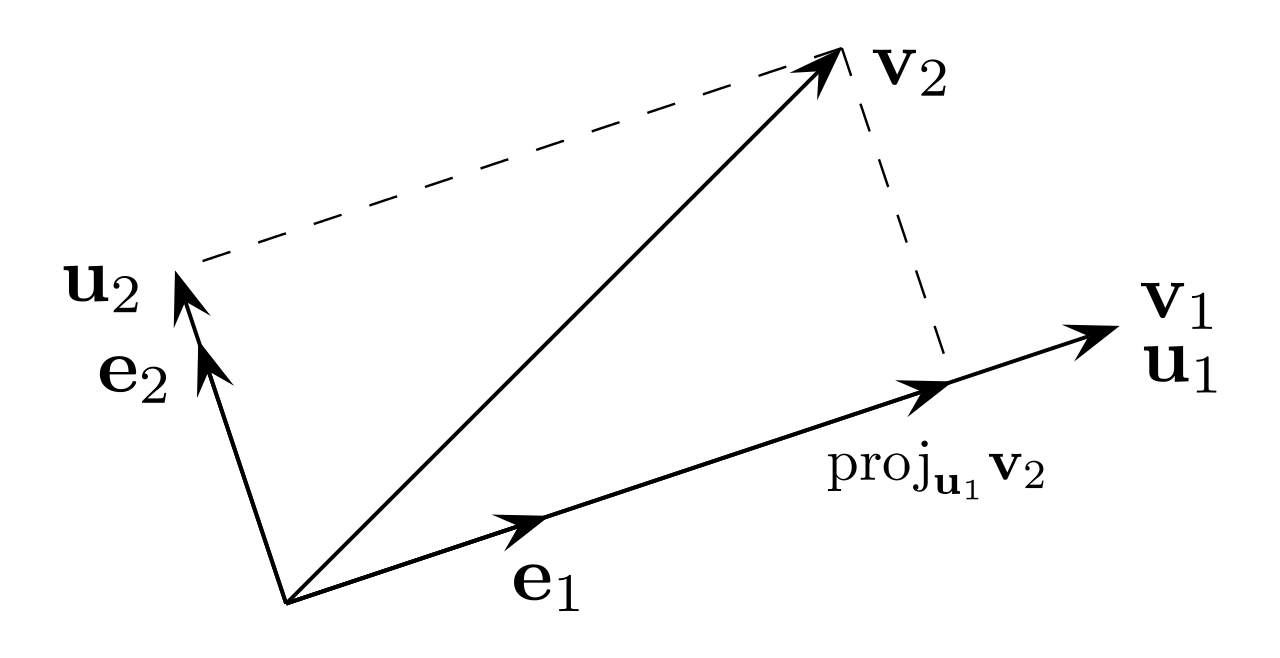
\includegraphics[scale=0.20]{graphics/15_6.png}

    \newpage

    \section{Liczby Stirlinga I i II rodzaju i ich interpretacja.}


    \begin{definition}
        \textbf{Liczby Stirling I rodzaju}.

        Dla dowolnego $n \geq 1$ mamy:
        \begin{enumerate}
            \item $c(0,0) = 1$
            \item $c(n,0) = c(0,n) = 0$
            \item $c(n,k) = c(n-1, k-1) + (n-1) * c(n-1, k)$
        \end{enumerate}
        W szczególności:
        \begin{enumerate}
            \item $c(n,n) = 1, c(n,1) = (n-1)!$
            \item $\sum^n_{k=0} c(n,k) = n!$
        \end{enumerate}

        \textbf{Interpretacja}: Przez $c(n,k)$ ($[^n_k]$) oznaczamy liczbę permutacji zbioru n-elementowego, które mają rozkład
        na dokładnie k cykli rozłącznych.
    \end{definition}

    \begin{definition}
        \textbf{Liczby Stirlinga II rodzaju}.

        Dla dowolnego $n \geq 1$ mamy:
        \begin{enumerate}
            \item $S(0,0) = 1$,
            \item $S(n,0) = S(0,n) = 0$,
            \item $S(n,k) = S(n-1, k-1) + k \times S(n-1, k)$.
        \end{enumerate}
        w szczególności  $S(n,n) = S(n,1) = 1$.\\

        \textbf{Interpretacja}: Przez $S(n,k)$ ($\{^n_k\}$) oznaczamy liczbę rozmieszczeń n rozróżnialnych kul na k nierozróżnialnych stosach w taki sposób,
        aby żaden stos nie był pusty.
    \end{definition}


    \newpage

    \section{Twierdzenia Eulera i Fermata; funkcja Eulera.}
    \begin{definition}
        \textbf{Funkcja Eulera (Tocjent)}

        Funkcja przypisująca każdej liczbie naturalnej liczbę liczb względnie pierwszych z nią i nie większych od niej.\newline $\sum_{m|n}^{} \varphi(m) = n$\newline

        \textbf{Własności}
        \begin{enumerate}
            \item $\varphi (n) \leq n - 1$  dla każdego $n>1$
            \item $\varphi (p) \leq p - 1$ dla każdego p będącego liczbą pierwszą
            \item $\varphi (mn) = \varphi (m)\varphi(n)$ jeśli NWD(m,n) = 1 (m i n względnie pierwsze)
            \item $\varphi(p^{k}) = p^{k-1} \cdot (p-1)$ jeśli p jest liczbą pierwszą
            \item $\varphi(n) = n
            \left (  1 - \frac{1}{p_1}\right)
            \left (  1 - \frac{1}{p_2}\right)
            \cdots
            \left (  1 - \frac{1}{p_n}\right)$
            gdzie $p_1, p_2, ..., p_n$ są czynnikami pierwszymi liczby n
            \item jeżeli $n = \prod_{i=1}^{k} p_i^{k_i}$ jest rozkładem liczby n na czynniki pierwsze $\varphi (n) = \prod_{i=1}^{k} \varphi \left( p_i^{k_i} \right )$
        \end{enumerate}
    \end{definition}

    \begin{definition}
        \textbf{Małe Twierdzenie Fermata}

        Jeżeli p jest liczbą pierwszą, to dla dowolnej liczby całkowitej a, liczba $a^{p}-a$ jest podzielna przez p.\newline
        \begin{enumerate}
            \item $a^{p-a} \equiv 0 \pmod p$\newline
        \end{enumerate}

        Jeśli p jest liczbą pierwszą, a a jest taką liczbą całkowitą, że liczby a i p są względnie pierwsze to $a^{p-1} - 1$ dzieli się przez p.\newline

        \begin{enumerate}
            \item$a^{p-1} - 1 \equiv \pmod p$
            \item$a^{p-1} \equiv 1 \pmod p$
        \end{enumerate}

    \end{definition}

    \begin{definition}
        \textbf{Twierdzenie Eulera}

        Jeżeli $m \in \mathbb{Z_{+}}$ oraz $a \in \mathbb{Z}$ są liczbami względnie pierwszymi to m dzieli liczbę $a^{\varphi(m)} - 1$, gdzie $\varphi (m)$ oznacza wartość funkcji Eulera.

        \begin{enumerate}
            \item $a^{\varphi (m)} \equiv 1 \pmod m$\newline
        \end{enumerate}

    \end{definition}
    \newpage

    \section{Konfiguracje i t-konfiguracje kombinatoryczne.}

    \begin{definition}
        \textbf{Konfiuracją kombinatoryczną} $B$ o parametrach $(n,k,r)$ nazywamy rodzinę $k$-elementowych podzbiorów w $X$, jeżeli każdy element $x \in X$ występuje w dokładnie $r$ podbiorach. Zachodzą warunki:
        \begin{enumerate}
            \item $n = |X|$
            \item $|B_i|=k \quad \forall i=1, \dots, b$
            \item $n \cdot r = b \cdot k$ \quad gdzie b to liczba k-elementowych podzbiorów zbioru n-elementowego
        \end{enumerate}
    \end{definition}

    \begin{theorem}
        Istnieje konfiguracja kombinatoryczna $B$ o parametrach $(n, k, r)$ wtedy i tylko wtedy, gdy:
        \begin{enumerate}
            \item $k | n\cdot r$
            \item $\frac{n\cdot r}{k}\leq {n\choose k}$
        \end{enumerate}

    \end{theorem}

    \begin{definition}
        Niech $X$ dowolny zbiór, $|X| = n.$ $B$ rodzina $k-$ podzbiorów $X$ jest
        \textbf{t-konfiguracją kombinatoryczną} o parametrach $(n, k, r_t)$ wtw gdy dla
        każdego $t-$podzbioru $T \subset X$ liczba bloków z $B$ zawierających $T$ jest
        równa $r_t$.
    \end{definition}

    \begin{theorem}
        Jeśli $B$ jest $t$-konfiguracją kombinatoryczną, to
        $B$ jest $s$-konfiguracją kombinatoryczną dla $s = 1, 2,\dots$ $t-1$.
        Uwagi:
        \begin{enumerate}
            \item $r_{t-1}$ $= r_t \cdot \frac{n-t+1}{k-t+1}$
            \item Jeżeli $B$ jest $t-$konfiguracją o parametrach $(n,k,r_t)$, to dla $1 \leq s \leq (t-1)$
            \begin{align*}
                r_s = r_t \cdot \frac{(n-s)(n-s-1)\dots(n-t+1)}{(k-s)(k-s-1)\dots(k-t+1)}
            \end{align*}
            \item Jeśli $B$ jest $t$-konfiguracją o parametrach $(n,k,r_t)$, to
            \begin{align*}
                (k-s)(k-s-1)\dots(k-t+1)|r_t(n-s)(n-s-1)\dots(n-t+1) \\ dla\  0\leq s \leq (t-1)
            \end{align*}
            warunek 3. dla $t\leq 2$ jest konieczny dla istnienia $t$-konfiguracji, ale nie wystarczający
        \end{enumerate}
    \end{theorem}

    \newpage

    \section{Cykl Hamiltona, obwód Eulera, liczba chromatyczna - definicje i twierdzenia.}

    \subsection{Cykl Hamiltona}
    \begin{definition}
        \textbf{Ścieżka Hamiltona}. Ścieżką Hamiltona w grafie $G$ nazywamy ścieżkę, która przechodzi przez wszystkie
        wierzchołki $G$.
    \end{definition}

    \begin{definition}
        \textbf{Cykl Hamiltona}. Powiemy, że graf $G$ ma cykl Hamiltona, jeśli istnieje w nim cykl przechodzący przez
        wszystkie wierzchołki. Taki graf nazwyamy hamiltonowskim.
    \end{definition}

    \begin{theorem}
        Niech $G = (V, E)$ będzie grafem o $n \geq 3$ wierzchołkach. Jeśli dla dwolonych różnych, niesąsiednich
        wierzchołków $u, v \in V$ zachodzi warunek $d(u) + d(v) \geq n$, to G jest hamiltonowski.
    \end{theorem}

    \begin{theorem}
        Jeśli $G$ jest grafem o $n \geq 3$ wierzchołkach w którym minimalny stopień wierzchołka wynosi co najmniej
        $\frac{n}{2}$, to G jest hamiltonowski.
    \end{theorem}

    \begin{theorem}
        Niech $G = (V, E)$ będzie grafem o $n \geq 2$ wierzchołkach i takim, że $d(u) + d(v) \geq n-1$ dla dwóch dowolnych
        różnych, niesąsiednich wierzchołków $u, v \in V$. Wtedy G ma ścieżkę hamiltona.
    \end{theorem}

    \subsection{Obwód Eulera}
    \begin{definition}
        \textbf{Droga Eulera}. Drogą Eulera w grafie $G$ nazywamy drogę $v_1, v_2, \dots, v_m$, w której każda krawędź grafu G użyta
        jest dokładnie raz.
    \end{definition}
    \begin{definition}
        \textbf{Obwód Eulera}. Jeśli w grafie $G$ istnieje droga Eulera, w której pierwszy i ostatni wierzchołek są identyczne, to nazywamy ją
        obwodem Eulera. Graf ten nazywamy wtedy eulerowskim.
    \end{definition}

    \begin{theorem}
        Niech $G$ będzie grafem spójnym. Wówczas następujące warunki są równowaźne:
        \begin{enumerate}
            \item G jest grafem eurelowskim,
            \item stopień każdego wierzchołka w G jest parzysty.
        \end{enumerate}
    \end{theorem}

    \begin{theorem}
        Niech G będzie grafem spójnym. Wówczas G ma drogę Eulera $\Leftrightarrow$ w G są dokładnie zero lub dwa wierzchołki
        stopnia nieparzystego.
    \end{theorem}

    \subsection{Liczba chromatyczna}
    \begin{definition}
        \textbf{Kolorowanie wierchołkowe}. Kolorowaniem wierzchołkowym grafu $G = (V, E)$ przy użyciu (co najwyżej) $k$
        kolorów nazywamy funkcję $c: V \rightarrow \{1, \dots, k\}$ spełniającą warunek
        $c(u) \neq c(v) ~~ \forall u, v \in V : uv \in E$.
    \end{definition}

    \begin{definition}
        \textbf{Liczba chromatyczna}. Liczbą chromatyczną grafu G nazywamy najmniejszą liczbę $k \in \mathbb{N}$, dla
        której istnieje kolorwanie wierzchołkowe G przy użyciu k kolorów. Oznaczamy $\chi(G)$.
        \begin{enumerate}
            \item $\chi(G) = 1 \Leftrightarrow |E(G)| = 0$
            \item $\chi(T) = 2$ dla każdego drzewa T o przynajmniej dwóch wierzchołkach
            \item $\chi(C_{2k}) = 2, \chi(C_{2k+1}) = 3$
            \item $\chi(K_n) = n$
        \end{enumerate}
    \end{definition}

    \begin{theorem}
        Niech G będzie dowolnym grafem. Wtedy $\chi(G) \leq d_{max}(G) + 1$.
    \end{theorem}

    \begin{theorem}
        Niech G będzie grafem spójnym. Wówczas $\chi(G) \leq d_{max}(G)$, o ile G nie jest grafem pełnym ani cyklem o
        nieparzystej liczbie wierzchołków.
    \end{theorem}

    \newpage

    \section{Algorytm Forda-Fulkersona wyznaczania maksymalnego przepływu.}

    \begin{definition}
        \textbf{Siecią przepływową} nazywamy zestaw $(V, \vec{E}, s, t, c)$, gdzie $(V, \vec{E})$ jest grafem
        skierowanym wraz z wyróżnionymi wierzchołkami $s$ - \textbf{źródłem} i $t$ - \textbf{ujściem} oraz
        \textbf{funkcją pojemności krawędzi} $c: ~ \vec{E} \rightarrow \mathbb{R}$.
    \end{definition}

    \begin{definition}
        \textbf{Przepływem} w sieci $(V, \vec{E}, s, t, c)$ nazywamy funkcję $f: \vec{E} \rightarrow \mathbb{R}$
        spełniającą następujące warunki:
        \begin{enumerate}
            \item $f(\vec{uv}) \leq c(\vec{uv})$  dla każdej krawędzi $\vec{uv} \in \vec{E}$,
            \item dla każdego ustalonego $v \in V\ \{s, t\}:$
            \begin{align*}
                \sum_{\vec{uv} \in \vec{E}} ~ f(\vec{uv}) ~~ = ~~ \sum_{\vec{vw} \in \vec{E}} ~ f(\vec{vw}).
            \end{align*}
        \end{enumerate}
        Liczbę $|f| =  \sum_{\vec{su}  \in \vec{E}} f(\vec{su}) = \sum_{\vec{wt} \in \vec{E}} f(\vec{wt})$ nazywamy
        \textbf{wartością przepływu} f.\\

        Przepływ f nazywamy \textbf{maksymalnym}, jeśli jego wartość jest największa spośród wszystkich przepływów w
        danej sieci.
    \end{definition}

    \begin{definition}
        Niech $(V, \vec{E}, s, t, c)$ będzie siecią przepływową oraz $f$ pewnym przepływem tej sieci. \textbf{Siecią rezydualną}
        nazywamy sieć $G_f = (V, E_f, s, t, c_f)$, gdzie $E_f = \vec{E} \cup \{\vec{vu}: \vec{uv} \in \vec{E}\}$ z funkcją
        pojemności określoną wzorem:
        \begin{align*}
            c_f(\vec{uv}) = c(\vec{uv}) - f(\vec{uv}) ~~ \text{dla} ~ \vec{uv} \in  \vec{E} ~  \text{t. że} ~ c(\vec{uv}) > 0
        \end{align*}
        \begin{align*}
            c_f(\vec{uv}) = f(\vec{uv}) ~~ \text{dla} ~ \vec{uv} \notin  \vec{E} ~  \text{t. że} ~ \vec{vu} \in \vec{E} \text{i} f(\vec{uv}) > 0
        \end{align*}
        oraz $c_f(\vec{uv}) = 0$ w pozostałych przypadkach.
    \end{definition}

    \begin{definition}
        \textbf{Ścieżką rozszerzającą} dla przepływu f nazywamy dowolną ścieżkę (skierowaną) $v_0 \rightarrow v_1 \rightarrow \cdots \rightarrow v_k$
        w sieci rezydualnej $G_f$ łączącą wierzchołki $v_0 = s$ i $v_k = t$, w której $c_f(\vec{v_i v_{i+1}}) > 0$ dla
        każdego $i = 0, \cdots, k-1$.
    \end{definition}

    \begin{theorem}
        \textbf{Algorytm Forda-Fulkersona}. W celu znalezienia maksymalnego przepływu $f$ w sieci przepływowej
        $(V, \vec{E}, s, t, c)$:
        \begin{enumerate}
            \item przyjmujemy początkowo dowolny (np. zerowy) przepływ $f$,
            \item budujemy sieć rezydualną $G_f$,
            \item dopóki w $G_f$ istnieje ścieżka rozszerzająca $P = v_0 \rightarrow v_1 \rightarrow \cdots \rightarrow v_k$
            określamy $c_p = min_{i = 0, \cdots, k-1} c_f(\vec{v_i v_{i+1}})$, a następni zwiększamy o $c_p$ wartość
            przepływu $f$ na krawędziach $\vec{v_i v_{i+1}}$ tej ścieżki i uaktualniamy wartośi funkcji $c_f$ sieci
            rezydualnej.
        \end{enumerate}
    \end{theorem}

    \begin{definition}
        \textbf{Przekrojem} w sieci przepływowej $(V, \vec{E}, s, t, c)$ nazywamy parę zbiorów $(S, T)$ spełniającą
        warunki:
        \begin{enumerate}
            \item $S \cup T = V$,
            \item $S \cap T = \emptyset$,
            \item $s \in S, t \in T$.
        \end{enumerate}

        \textbf{Pojemnością} przekroju $(S,T)$ nazywamy liczbę
        \begin{align*}
            c(S, T) = \sum_{(u,v) \in \vec{E} \cap (S \times T)} c(\vec{uv}).
        \end{align*}
    \end{definition}

    \begin{theorem}
        Niech $(V, \vec{E}, s, t, c)$ będzie siecią przepływową. Wówczas \textbf{maksymalna wartość przepływu jest
        jest równa minimalnej pojemności} przekroju w tej sieci.
    \end{theorem}

    \newpage

    \section{Rozwiązywanie równań rekurencyjnych przy użyciu funkcji tworzących (generujących) oraz przy użyciu
    równania charakterystycznego.}

    \begin{definition}
        \textbf{Liniowym równaniem rekurencyjnym rzędu r} (o stałych współczynnikach) nazywamy równanie postaci:
        \begin{align*}
            x_{n+r} = c_1 x_{n+r-1} +  \cdots + c_r x_n + f(n)
        \end{align*}
        w którym $c_i  \in \mathbb{R}, c_r \neq 0$  oraz $f:  \mathbb{N} \rightarrow \mathbb{R}$ jest dowolną funkcją.
        Jeśli funkcja f jest stale równa zero, to powyższe równanie nazywamy \textbf{jednorodnym}.
    \end{definition}

    \begin{definition}
        \textbf{Rozwiązaniem szczególnym} równania nazywamy dowolny ciąg $(x_n)$ spełniający zależność rekurencyjną.
        Dla każdego równania jednorodnego rozwiązanie szczególnym jest ciąg stały równy zero.

        \textbf{Rozwiązaniem ogólnym} równania nazywamy wzór ogólny (zależny od pewnych parametrów) pozwalający
        wyznaczyć wszystkie rozwiązania szczególne.
    \end{definition}

    \subsection{Funkcje tworzące.}
    \begin{definition}
        \textbf{Funkcją tworzącą} (generujacą) ciągu $(a_n)$ nazywamy szereg
        \begin{align*}
            \sum_{n=0}^{\infty} a_n x^n.
        \end{align*}
        Jest to tylko inny zapis ciągu (wyraz $a_n$ to współczynnik przy $x^n$) - nie interesują nas kwestie zbieżności,
        podstawiania wartości za x, ciągłości/różniczkowalności funkcji określonej takim szeregiem itd.

        Jeżeli jednak funkcja tworząca pewnego ciągu "wygląda" jak zbieżny szereg określający funkcję znaną z analizy
        to możemy używać skróconego zapisu, np. $\sum_{n=0}^{\infty} \frac{1}{n!} x^n = e^x$.
    \end{definition}

    \begin{theorem}
        \textbf{Operacje na funkcjach tworzących}.
        \begin{enumerate}
            \item Funkcje tworzące można \textbf{dodawać,odejmować i mnożyć przez liczbę} - odpowiadają temu operacje
            dodawania, odejmowania i mnożenia przez liczbę wyrazów ciągu.
            \item \textbf{Mnożeniu dwóch funkcji tworzących} odpowiada operacja "splotu", tzn. jeśli
            $A(x) =  \sum_{n=0}^{\infty} a_n x^n$ i $B(x) = \sum_{n=0}^{\infty} b_n x^n$, to
            $A(x) * B(x) = \sum_{n=0}^{\infty} c_n x^n$, gdzie $c_n = \sum_{k=0}^n a_k b_{n-k}$.
            \item Jeśli funkcja tworząca A(x) ma "element odwrotny", tzn. taką funkcję tworzącą B(x) dla której
            $A(x) * B(x) = 1$, to mówimy że A(x) jest \textbf{odwracalna} i piszemy $\frac{1}{A(x)} = B(x)$.
            \item \textbf{Mnożeniu funkcji} tworzącej \textbf{przez x} odpowiada przesunięcie ciągu (dopisanie na początek
            wyrazu zerowego). Operajcją odwrotną jest odjęcie wyrazu zerowego i podzielenie przez x.
            \item Funkcje tworzące można \textbf{różniczkować} według wzoru:
            \begin{align*}
                (\sum_{n=0}^{\infty} a_n x^n)' = \sum_{n=1}^{\infty} n a_n x^{n-1} = \sum_{n=0}^{\infty} (n+1) a_{n+1} x^n
            \end{align*}
            \item Zachodzą wzory na \textbf{pochodne} znane z analizy, np. $(A(x) * B(x))' = A'(x)B(x) + A(x)B'(x)$.
            \item Operacja \textbf{"całkowania"} (odwrotna do różniczkowania):
            \begin{align*}
                \int (\sum_{n=0}^{\infty} a_n x^n) = \sum_{n=0}^{\infty} \frac{a_n}{n+1} x^{n+1} = \sum_{n=0}^{\infty} \frac{a_n - 1}{n} x^n
            \end{align*}
            Wyraz $a_n$ można "odzyskać" z funkcji tworzącej A(x) wykonując jej n-krotne różniczkowanie.
        \end{enumerate}
    \end{theorem}

    \begin{theorem}
        Dla dowolnej liczby naturalnej $m \geq 1$ zachodzi wzór:
        \begin{align*}
            \frac{1}{(1-x)^m} ~ = ~ \sum_{n=0}^{\infty} \binom{n+m-1}{n} x^n.
        \end{align*}

        Dla dowolneego $\alpha \in \mathbb{R}$ oraz $|x| < 1$ zachodzi wzór:
        \begin{align*}
            (1+x)^{\alpha} ~ - ~ \sum_{n=0}^{\infty} \binom{\alpha}{n} x^n
        \end{align*}
    \end{theorem}

    \subsection{Równanie charakterystyczne.}
    \begin{definition}
        \textbf{Równanie charakterystyczne} równania rekurencyjnego. Weźmy równanie rekurencyjne jednorodne
        \begin{align*}
            a_n = A a_{n-1} + B a_{n-2}
        \end{align*}
        gdzie dane są współczynniki A, B. Załóżmy, że ma ono rozwiązanie postaci $a_n = t^n$. Podstawiając otrzymujemy:
        \begin{align*}
            t^n = A t^{n-1} + B t^{n-2}.
        \end{align*}
        Dzielimy obie strony przez $t^{n-2}$:
        \begin{align*}
            t^2 = A t^1 + B
        \end{align*}
        \begin{align*}
            t^2 - A t^1 - B = 0.
        \end{align*}
        Równanie to nazywamy równaniem charakterystycznym równania rekurencyjnego. W tym przypadku jest to równanie kwadratowe.

        Jeżeli nie ma ono pierwiastków podwójnych, wówczas:
        \begin{align*}
            a_n = C r_1^n + D r_2^n.
        \end{align*}
        Jeżeli ma pierwiastki podwójne, to:
        \begin{align*}
            a_n = (C + Dn) r_1^n.
        \end{align*}
        C i D są dowolnymi stałymi a $r_{1}$ i $r_{2}$ są pierwiastkami równania charakterystycznego. Jeżeli dane jest
        $a_{1}$ i $a_{2}$ wówczas można łatwo ułożyć układ równań i otrzymać ich wartość.
    \end{definition}

    \newpage

    \section{Ciąg i granica ciągu liczbowego, granica funkcji.}

    \subsection{Ciągi.}

    \begin{definition}
        \textbf{Ciąg liczbowy}. Ciągiem liczbowym nazywamy funkcję $\mathbb{N} \rightarrow \mathbb{R}$. Wartość tej
        funkcji dla liczby naturalnej $n$ nazywamy $n$-tym wyrazem ciągu i oznaczamy przez $a_n$, $b_n$ itp. Ciągi o
        takich wyrazachoznaczamy odpowiednio przez $(a_n)$, $(b_n)$  itp. Zbiór wyrazów ciągu $(a_n)$, tj.
        $\{a_n : n  \in \mathbb{N}\}$ oznaczamy krótko przez  $\{a_n\}$.
    \end{definition}

    \begin{definition}
        \textbf{Granica właściwa ciągu}. Ciąg $(a_n)$ jest zbieżny do granicy właściwej $a \in \mathbb{R}$, co zapisujemy:
        \begin{align*}
            lim_{n  \rightarrow \infty} ~ a_n = a
        \end{align*}
        wtedy i tylko wtedy, gdy
        \begin{align*}
            \forall \varepsilon > 0 ~~ \exists  n_0 \in \mathbb{N} ~~ \forall n \in \mathbb{N} ~~~ [(n > n_0) \Rightarrow (|a_n - a| < \varepsilon)]
        \end{align*}
    \end{definition}

    \begin{definition}
        \textbf{Granice niewłaściwe ciągu}.

        Ciąg $(a_n)$ jest zbieżny do granicy niewłaściwej $\infty$, co zapisujemy:
        \begin{align*}
            lim_{n \rightarrow \infty} ~ a_n = \infty
        \end{align*}
        wtedy i tylko wtedy, gdy:
        \begin{align*}
            \forall \varepsilon > 0 ~~ \exists  n_0 \in \mathbb{N} ~~ \forall n \in \mathbb{N} ~~~ [(n > n_0) \Rightarrow (a_n > \varepsilon)]
        \end{align*}

        Ciąg $(a_n)$ jest zbieżny do granicy niewłaściwej $-\infty$, co zapisujemy:
        \begin{align*}
            lim_{n \rightarrow \infty} a_n = -\infty
        \end{align*}
        wtedy i tylko wtedy, gdy:
        \begin{align*}
            \forall \varepsilon < 0 ~~ \exists  n_0 \in \mathbb{N} ~~ \forall n \in \mathbb{N} ~~~ [(n > n_0) \Rightarrow (a_n < \varepsilon)]
        \end{align*}
    \end{definition}

    \begin{theorem}
        \textbf{O ograniczoności ciągu zbieżnego}. Jeśli ciąg jest zbieżny do granicy właściwej, to jest ograniczony.
    \end{theorem}

    \begin{theorem}
        \textbf{O równoważności granic.}
        \begin{align*}
            lim_{n \rightarrow \infty} ~ a_n = 0 ~~ \Leftrightarrow ~~ lim_{n \rightarrow \infty} ~ |a_n| = 0.
        \end{align*}
    \end{theorem}

    \begin{theorem}
        \textbf{O dwóch ciągach}. Jeśli ciągi $(a_n)$, $(b_n)$ spełniają warunki:
        \begin{enumerate}
            \item $a_n \leq b_n ~~~ \forall n \geq n_0$
            \item $lim_{n \rightarrow \infty} a_n = \infty$
        \end{enumerate}
        to
        \begin{align*}
            lim_{n \rightarrow \infty} ~ b_n = \infty.
        \end{align*}

        Prawdziwe jest także analogiczne twierdzenie dla ciągów zbieżnych do granicy niewłaściwej $-\infty$.
    \end{theorem}

    \begin{theorem}
        \textbf{O trzech ciągach}. Jeśli ciągi $(a_n)$, $(b_n)$, $(c_n)$ spełniają warunki:
        \begin{enumerate}
            \item $a_n \leq b_n \leq c_n ~~~ \forall n \geq n_0$
            \item $lim_{n  \rightarrow \infty} a_n = lim_{n \rightarrow \infty} c_n = b$
        \end{enumerate}
        to
        \begin{align*}
            lim_{n \rightarrow \infty} ~ b_n = b.
        \end{align*}
    \end{theorem}

    \begin{theorem}
        \textbf{O ciągu monotonicznym i ograniczonym}. Jeżeli ciąg $(a_n)$ jest niemalejący dla $n \geq n_0$ oraz
        ograniczony z góry, to jest zbieżny do granicy właściwej $sup\{a_n : n \geq n_0\}$.

        Prawdziwe jest także analogiczne twierdzenie dla ciągu nierosnącego i ograniczonego z dołu.
    \end{theorem}

    \subsection{Funkcje.}

    \begin{definition}
        \textbf{Heinego granicy właściwej funkcji w punkcie}. Niech $x_0 \in \mathbb{R}$ oraz niech funkcja $f$ będzie
        określona przynajmniej na sąsiedztwie $S(x_0)$. Liczba $g$ jest granicą właściwą funkcji $f$ w punkcie $x_0$, co
        zapisujemy
        \begin{align*}
            lim_{x \rightarrow x_0} ~ f(x) = g
        \end{align*}
        wtedy i tylko wtedy, gdy
        \begin{align*}
            \forall_{(x_n): ~ \{x_n\} \subset S(x_0)} ~~ [(lim_{n \rightarrow \infty} x_n = x_0) \Rightarrow (lim_{n \rightarrow \infty} f(x_n) = g)].
        \end{align*}
    \end{definition}

    \begin{definition}
        \textbf{Cauchy'ego granicy właściwej funkcji w punkcie}. Niech $x_0 \in \mathbb{R}$ oraz niech funkcja $f$ będzie
        określona przynajmniej na sąsiedztwie $S(x_0)$. Liczba $g$ jest granicą właściwą funkcji $f$ w punkcie  $x_0$,
        co zapisujemy
        \begin{align*}
            lim_{x \rightarrow x_0} ~ f(x)  = g
        \end{align*}
        wtedy i tylko wtedy, gdy
        \begin{align*}
            \forall \varepsilon > 0 ~~ \exists \delta > 0 ~~ \forall  x \in S(x_0)  ~~~ [(|x - x_0| <  \delta) \Rightarrow (|f(x) - g| < \varepsilon)].
        \end{align*}
        \hfill \\

        Funkcja $f$ ma granicę niewłaściwą $\infty$ w punkcie $x_0$ wtedy i tylko wtedy, gdy
        \begin{align*}
            \forall \varepsilon > 0 ~~ \exists \delta > 0 ~~ \forall  x \in S(x_0)  ~~~ [(|x - x_0| <  \delta) \Rightarrow (f(x) > \varepsilon)].
        \end{align*}

    \end{definition}

    \begin{theorem}
        \textbf{O nieistnieniu granicy funkcji w punkcie}. Jeśli istnieją ciągi $(x'_n)$, $(x''_n)$ spełniające warunki:
        \begin{enumerate}
            \item $lim_{n \rightarrow \infty} x'_n = x_0$, przy czym $x'_n \neq x_0 ~~ \forall n \in \mathbb{N}$
            oraz $lim_{n \rightarrow \infty}  ~ f(x'_n) = g'$,
            \item $lim_{n \rightarrow \infty} x''_n = x_0$, przy czym $x''_n \neq x_0 ~~ \forall n \in \mathbb{N}$
            oraz $lim_{n \rightarrow \infty}  ~ f(x''_n) = g''$,
            \item $g' \neq g''$,
        \end{enumerate}
        to granica $lim_{x \rightarrow x_0} ~ f(x)$ nie istnieje (właściwa ani niewłaściwa).
    \end{theorem}

    \begin{theorem}
        \textbf{Warunek konieczny i wystarczajacy istnienia granicy}. Funckja $f$ ma w punkcie $x_0$ granicę
        właściwą (niewłaściwą) wtedy i tylko wtedy, gdy
        \begin{align*}
            lim_{x \rightarrow x^{-}_0}  ~ f(x) ~ = ~ lim_{x \rightarrow x^{+}_0}  ~ f(x)
        \end{align*}
        Wspólna wartość granic jednostronnych jest wtedy granicą funkcji.
    \end{theorem}

    \begin{theorem}
        \textbf{O niesitnieniu granicy funkcji w nieskończoności}. Jeżeli istnieją ciągi $(x'_n)$, $(x''_n)$
        spełniające warunki:
        \begin{enumerate}
            \item $lim_{n \rightarrow \infty} ~ x'_n = \infty $ oraz $ lim_{n \rightarrow \infty} ~ f(x'_n) = g'$,
            \item $lim_{n \rightarrow \infty} ~ x''_n = \infty $ oraz $ lim_{n \rightarrow \infty} ~ f(x''_n) = g''$,
            \item $g' \neq g''$,
        \end{enumerate}
        to nie istnieeje granica $lim_{x \rightarrow x_0} ~ f(x)$ (właściwa ani niewłaściwa).
    \end{theorem}

    \begin{theorem}
        \textbf{O dwóch funkcjach}. Jeśli funkcje $f$ i $g$ spełniają warunki:
        \begin{enumerate}
            \item $f(x) \leq g(x) ~~ \forall x \in S(x_0)$,
            \item $lim_{x \rightarrow x_0} ~ f(x) = \infty$,
        \end{enumerate}
        to
        \begin{align*}
            lim_{x \infty x_0} ~ g(x) = \infty.
        \end{align*}
    \end{theorem}

    \begin{theorem}
    	\textbf{Granice specjalne}
    	\setlength{\jot}{10pt}
    	\begin{align*}
    		&\lim_{x \to +\infty} a^{x} x^{\alpha} \stackrel{[0 \cdot \infty]}{=}  \text{0 dla a} \in (0, 1), \alpha \geq 0 \\
    		&\lim_{x \to 0} \frac{\sin{x}}{x} \stackrel{[\frac{0}{0}]}{=} \text{1 oraz}    \lim_{x \to 0} \frac{\arcsin{x}}{x} \stackrel{[\frac{0}{0}]}{=} 1\\
    		&\lim_{x \to 0} (1 + x)^{\frac{1}{x}} \stackrel{1^{\infty}}{=} \text{e oraz}   \lim_{x \to \infty} (1 + x)^{\frac{1}{x}} \stackrel{\infty^{0}}{=} 1 \\
    		&\lim_{x \to 0} \frac{a^x -1}{x} \stackrel{[\frac{0}{0}]}{=} \ln{a} \text{ dla  a $>$ 0, w szczególności } \lim_{x \to 0} \frac{e^x -1}{x} \stackrel{[\frac{0}{0}]}{=} 1 \\
    		&\lim_{x \to 0} \frac{\log_{a}(1 + x)}{x} \stackrel{[\frac{0}{0}]}{=} \frac{1}{\ln{a}} \text{, w szczególności } \lim_{x \to 0} \frac{\ln(1 + x)}{x} \stackrel{[\frac{0}{0}]}{=} 1 \\
    		&\lim_{x \to \pm \infty} (1 + \frac{a}{x})^{x} \stackrel{[1^{\infty}]}{=} e^{a} \text{, dla a} \in \mathbb{R} \\
    		&\lim_{x \to 0} \frac{(1 + x)^a - 1}{x} \stackrel{[\frac{0}{0}]}{=} \text{a, dla a} \in \mathbb{R}
    	\end{align*}
    \end{theorem}

    \begin{theorem}
        \textbf{Reguła de L'Hostpiala}. Jeżeli funkcja $f$ i  $g$ spełniają warunki:
        \begin{enumerate}
            \item $lim_{x \rightarrow x_0} f(x) = lim_{x \rightarrow x_0} g(x) = 0 ~~ (\infty)$, przy czym $g(x) \neq 0$ dla $x \in S(x_0)$
            \item istnieje granica $lim_{x \rightarrow x_0} \frac{f'(x)}{g'(x)}$ (właściwa lub niewłaściwa),
        \end{enumerate}
        to
        \begin{align*}
            lim_{x \rightarrow x_0} \frac{f(x)}{g(x)} = lim_{x \rightarrow x_0} \frac{f'(x)}{g'(x)}
        \end{align*}
    \end{theorem}

    \newpage

    \section{Ciągłość i pochodna funkcji. Definicja i podstawowe twierdzenia.}

    \subsection{Ciągłość.}

    \begin{definition}
        \textbf{Funkcja ciągła w punkcie}. Niech $x_0 \in \mathbb{R}$ oraz niech funkcja $f$ będzie określona przynajmniej
        na otoczeniu $O(x_0)$. Funkcja $f$ jest ciągła w ounkcie $x_0$ wtedy i tylko wtedy, gdy
        \begin{align*}
            lim_{x \rightarrow x_0} ~ f(x) = f(x_0).
        \end{align*}
        \hfill \\

        \textbf{Funkcja jest ciągła na zbiorze}, jeżeli jest ciągła w każdym punkcie tego zbioru.
    \end{definition}

    \begin{theorem}
        \textbf{Warunek konieczny i wystarczający ciągłości funkcji}. Funckja jest ciągła w punkcie wtedy i tylko wtedy,
        gdy jest w tym punkcie ciągła lewostronnie i prawostronnie.
    \end{theorem}

    \begin{definition}
        \textbf{Nieciągłość funkcji}. Niech $x_0 \in \mathbb{R}$ oraz niech funkcja $f$ będzie określona przynajmniej
        na otoczeniu $O(x_0)$. Funkcja $f$ jest nieciągła w punkcie $x_0$ wtedy i tylko wtedy, gdy nie istnieje
        granica $lim_{x \rightarrow x_0} ~ f(x)$ albo gdy $lim_{x \rightarrow x_0} ~ f(x) \neq f(x_0)$.
        \hfill \\

        \textbf{Nieciągłość pierwszego rodzaju}. Jeżeli istnieją granice skończone $lim_{x \rightarrow x^{-}_0 ~ f(x)}$,
        $lim_{x \rightarrow x^{+}_0} ~ f(x)$ oraz
        \begin{align*}
            lim_{x \rightarrow x^{-}_0} ~ f(x) \neq  f(x_0) ~~~ \text{lub} ~~~ lim_{x \rightarrow x^{+}_0} ~ f(x) \neq f(x_0).
        \end{align*}
        Mówimy, że funkcja $f$ ma w punkcie $x_0$ nieciągłość pierwszego rodzaju typu "skok", jeżeli spełnia warunek
        \begin{align*}
            lim_{x \rightarrow x^{-}_0} ~ f(x) ~ \neq ~ lim_{x \rightarrow x^{+}_0} ~ f(x).
        \end{align*}
        Mówi, że funkcja $f$ ma w punkcie $x_0$ nieciągłość pierwszego rodzaju typu "luka", jeżeli spełnia warunek
        \begin{align*}
            lim_{x \rightarrow x^{-}_0} ~ f(x) ~ = ~ lim_{x \rightarrow x^{+}_0} ~ f(x) ~ \neq ~ f(x_0).
        \end{align*}
        \hfill \\

        \textbf{Nieciągłość drugiego rodzaju}. Jeżeli co najmniej jedna z granic
        \begin{align*}
            lim_{x \rightarrow x^{-}_0} ~ f(x), ~~ lim_{x \rightarrow x^{+}_0} ~ f(x)
        \end{align*}
        nie istnieje lub jest niewłaściwa.
    \end{definition}

    \begin{theorem}
        \textbf{Weierstrassa o ograniczoności funkcji ciągłej}. Jeżeli funkcja jest ciągła na przedziale domkniętym
        i ograniczonym, to jest na nim ograniczona.
    \end{theorem}

    \begin{theorem}
        \textbf{Weierstrassa o osiąganiu kresów}. Jeżeli funkcja $f$ jest ciągła na przedziale domkniętym $[a, b]$,to
        \begin{align*}
            \exists c \in [a,b] ~~ f(c) = ~ inf_{x \in [a,b]} ~ f(x) ~~ \text{oraz} ~~ \exists d \in [a,b] ~~ f(d) = ~ sup_{x \in [a,b]} ~ f(x)
        \end{align*}
    \end{theorem}

    \begin{theorem}
        \textbf{Darboux o przyjmowaniu wartości pośrednich}. Jeżeli funkcja $f$ jest ciągła na przedziale $[a,b]$ oraz
        spełnia warunek $f(a) < f(b)$, to
        \begin{align*}
            \forall w \in (f(a, f(b))) ~ \exists c \in (a,b) ~~ f(c) = w.
        \end{align*}
    \end{theorem}


    \subsection{Pochodna.}

    \begin{definition}
        \textbf{Iloraz różnicowy}. Niech  $x_0 \in \mathbb{R}$ oraz niech funkcja $f$ będzie określona przynajmniej
        na otoczeniu $O(x_0, r)$, gdzie $r > 0$. Ilorazem różnicowym funkcji $f$ w punkcie $x_0$  odpowiadającym przyrostowi
        $\Delta x$, gdzie $0 < |\Delta x| < r$, zmiennej niezależnej nazywamy liczbę
        \begin{align*}
            \frac{\Delta f}{\Delta x} \stackrel{def}{=} \frac{f(x_0 + \Delta x) - f(x_0)}{\Delta x}
        \end{align*}
    \end{definition}

    \begin{definition}
        \textbf{Pochodna właściwa funkcji}. Niech $x_0 \in \mathbb{R}$ oraz niech funkcja $f$ będzie określona przynajmniej
        na otoczeniu $O(x_0)$. Pochodną właściwą funkcji $f$ w punkcie $x_0$ nazywamy granicę właściwą
        \begin{align*}
            f'(x_0) ~ \stackrel{def}{=} ~ lim_{x \rightarrow x_0} ~ \frac{f(x) - f(x_0)}{x - x_0}
        \end{align*}

        Inaczej mówiąc pochodna funkcji $f$ jest granicą ilorazu różnicowego gdy $\Delta x \rightarrow \infty$. Mamy zatem
        \begin{align*}
            f'(x_0) ~ \stackrel{def}{=} ~ lim_{\Delta x \rightarrow \infty} ~ \frac{f(x_0 + \Delta x) - f(x_0)}{\Delta x}
        \end{align*}
    \end{definition}

    \begin{theorem}
        \textbf{Warunek konieczny istnienia pochodnej właściwej funkcji}. Jeżeli funkcja ma pochodną właściwą w punkcie,
        to jest ciągła w tym punkcie. Implikacja odwrotna nie jest prawdziwa.
    \end{theorem}

    \begin{definition}
        \textbf{Pochodne jednostronne właściwe funkcji}. Niech $x_0 \in \mathbb{R}$ oraz niech funkcja $f$ będzie
        określona przynajmniej na otoczeniu  $O(x^{-}_0)$. Pochodną lewostronną właściwą funkcji $f$ w punkcie $x_0$
        nazywamy granicę właściwą
        \begin{align*}
            f'_{-}(x_0) ~ \stackrel{def}{=} ~ lim_{x \rightarrow x^{-}_0} ~ \frac{f(x) - f(x_0)}{x - x_0}
        \end{align*}
        Analogicznie definiujemy $f'_{+}(x_0)$.\\

        Jeżeli funkcja ma w punkcie pochodną lewostronną (prawostronną) właściwą, to jest w nim ciągła lewostronnie
        (prawostronnie).
    \end{definition}

    \begin{definition}
        \textbf{Pochodna funkcji na zbiorze}. Funkcja ma pochodną właściwą na zbiorze wtedy i tylko wtedy, gdy ma pochodną
        właściwą w każdym punkcie tego zbioru.
    \end{definition}

    \begin{definition}
        \textbf{Pochodna niewłaściwa funkcji}. Niech $f$ będzie funkcją ciągłą w punkcie $x_0 \in \mathbb{R}$. Funkcja
        $f$ ma w punkcie $x_0$ pochodną niewłaściwą wtedy i tylko wtedy, gdy
        \begin{align*}
            lim_{x \rightarrow  x_0} ~ \frac{f(x) - f(x_0)}{x - x_0} = \infty ~~ \text{albo} ~~ lim_{x  \rightarrow x_0} ~ \frac{f(x) - f(x_0)}{x - x_0} = -\infty
        \end{align*}
        Podobnie definiujemy pochodne niewłaściwe jednostronne.
    \end{definition}

    \begin{theorem}
        \textbf{Zastosowanie różniczki do obliczeń przybliżonych}. Jeżeli funkcja $f$ ma pochodną właściwą w punkcie
        $x_0$, to
        \begin{align*}
            f(x_0 + \Delta x) \approx f(x_0) + f'(x_0)\Delta x
        \end{align*}
        Przy czym błąd, jaki popełniamy zastępując przyrost funkcji
        \begin{align*}
            \Delta f = f(x_0 \Delta x) - f(x_0)
        \end{align*}
        jej różniczką $df = f'(x_0)\Delta x$, dąży szybciej do zera niż przyrost zmiennej niezależnej $\Delta x$, tzn.
        \begin{align*}
            lim_{\Delta  x  \rightarrow 0} \frac{\Delta f - df}{\Delta  x} = 0.
        \end{align*}
    \end{theorem}

    \begin{theorem}
        \textbf{Rolle'a}. Jeśli funkcja $f$ spełnia warunki:
        \begin{enumerate}
            \item jest ciągła na $[a,b]$
            \item ma pochodną właściwą lub niewłaściwą na $(a,b)$,
            \item $f(a) = f(b)$,
        \end{enumerate}
        to istnieje punkt $c \in (a,b)$ taki, że:
        \begin{align*}
            f'(c) = 0.
        \end{align*}
    \end{theorem}

    \begin{theorem}
        \textbf{Lagrange'a}. Jeżeli funkcja $f$ spełnia warunki:
        \begin{enumerate}
            \item jest ciągła na $[a,b]$,
            \item ma pochodną właściwą lub niewłaściwą na $(a,b)$,
        \end{enumerate}
        to istnieje punkt $c \in (a,b)$ taki, że
        \begin{align*}
            f'(c) = \frac{f(b)-f(a)}{b-a}
        \end{align*}
    \end{theorem}

    \newpage

    \section{Ekstrema funkcji jednej zmiennej. Definicje i twierdzenia.}

    \begin{definition}
        \textbf{Minimum lokalne funkcji}. Funkcja $f$ ma w punkcie $x_0 \in \mathbb{R}$ minimum lokalne, jeżeli:
        \begin{align*}
            \exists \delta > 0 ~ \forall x \in S(x_0, \delta) ~~ f(x) \geq f(x_0).
        \end{align*}
        Analogicznie definiujemy \textbf{maksimum lokalne}.\\

        \textbf{Minimum lokalne jest właściwe}, jeżeli:
        \begin{align*}
            \exists \delta > 0 ~ \forall x \in S(x_0, \delta) ~~ f(x) > f(x_0).
        \end{align*}
        Analogicznie definiujemy \textbf{maksimum lokalne właściwe}.\\
    \end{definition}

    \begin{theorem}
        \textbf{Fermata, warunek konieczny istnienia ekstremum}. Jeżeli funkcja $f$ ma:
        \begin{enumerate}
            \item esktremum lokalne w punkcie $x_0$,
            \item pochodną $f'(x_0)$,
        \end{enumerate}
        to
        \begin{align*}
            f'(x_0) = 0.
        \end{align*}
    \end{theorem}

    \begin{theorem}
        \textbf{I warunek wystarczający istnienia ekstremum}. Jeżeli funkcja $f$ spełnia warunki:
        \begin{enumerate}
            \item $f'(x_0) = 0$,
            \item $\exists \delta > 0
            \left\{\begin{matrix}
                       f'{x} > 0 ~~ \forall x \in  S(x^{-}_0, \delta), \\
                       f'{x} < 0 ~~ \forall x \in  S(x^{+}_0, \delta),
            \end{matrix}\right.$
        \end{enumerate}
        to w punkcie $x_0$ ma maksimum lokalne właściwe. Analogicznie dla minimum.
    \end{theorem}

    \begin{theorem}
        \textbf{II warunek wystarczający istnienia ekstremum}. Jeżeli funkcja $f$ spełnia warunki:
        \begin{enumerate}
            \item $f'(x_0) = f''(x_0) = \dots = f^{(n-1)}(x_0) = 0$,
            \item $f^{(n)}(x_0) < 0$,
            \item $n$ jest liczbą parzystą, gdzie $n \geq 2$,
        \end{enumerate}
        to w punkcie $x_0$ ma maksimum lokalne właściwe. Analogicznie dla minimum,
    \end{theorem}

    \newpage

    \section{Całka Riemanna funkcji jednej zmiennej.}

    \begin{definition}
        \textbf{Całka oznaczona Riemanna}. Niech funkcja $f$ będzie ograniczona na przedziale $[a,b]$. Całkę oznaczoną
        Riemanna z funkcji  $f$  na przedziale $[a,b]$ definiujemy wzorem
        \begin{align*}
            \int_{a}^{b} f(x) \,dx ~~ \stackrel{def}{=} ~~ lim_{\delta(P)  \rightarrow 0} \sum_{k=1}^{n} f(x^{*}_k) \Delta x_k,
        \end{align*}
        o ile po prawej stronie znaku równości granica jest właściwa oraz nie zależy od sposoby podziałów $P$ przedziału
        $[a,b]$ ani od sposobów wyboru punktów pośrednich $x^{*}_k$, gdzie $1 \leq k \leq n$. Ponadto przyjmujemy
        \begin{align*}
            \int_a^a f(x)\,dx ~ \stackrel{def}{=} ~ 0 ~~~~ \text{oraz} ~~~~ \int_b^a f(x)\,dx ~ \stackrel{def}{=} ~ - ~ \int_a^b f(x) \,dx ~~ \text{dla} ~ a < b
        \end{align*}
        Funkcję, dla której istnieje całka Riemanna, nazywamy całkowalną.
    \end{definition}

    \begin{theorem}
        \textbf{Warunek wystarczający całkowalności funkcji}. Jeżeli funkcja $f$ jest ograniczona na przedziale $[a,b]$
        i ma na tym przedziale skończoną liczbę punktów nieciągłości I rodzaju, to jest na nim całkowalna.
    \end{theorem}

    \begin{theorem}
        \textbf{Obliczanie całek przy pomocy sumy całkowej podziału równomiernego}. Jeżeli funkcja $f$ jest całkowalna
        na przedziale $[a,b]$, to
        \begin{align*}
            \int_{a}^b f(x) \, dx ~ = ~ lim_{n \rightarrow \infty} [\frac{b - a}{n} \sum_{k=1}^n f (a + k \frac{b - a}{n})]
        \end{align*}
    \end{theorem}

    \begin{theorem}
        \textbf{Newtona - Leibniza, główne twierdzenie rachunku całkowego}. Jeżeli funkcja $f$ jest ciągła na przedziale
        $[a,b]$, to
        \begin{align*}
            \int_a^b f(x) \,dx ~ = ~ F(b) - F(a) ~ = ~ [F(x)]_a^b,
        \end{align*}
        gdzie F oznacza dowolną funkcję pierwotną funkcji $f$  na tym przedziale.
    \end{theorem}

    \newpage

    \section{Pochodne cząstkowe funkcji wielu zmiennych; różniczkowalność i różniczka funkcji.}

    \begin{definition}
        \textbf{Pochodne cząstkowe}. Niech funkcja $f$ będzie określona przynajmniej na otoczeniu punktu $(x_0, y_0)$.
        Pochodną cząstkową pierwszego rzędu funkcji $f$ względem $x$ w punkcie $(x_0, y_0)$ określamy wzorem:
        \begin{align*}
            \frac{\partial f}{\partial x}(x_0, y_0)  \stackrel{def}{=} lim_{\Delta x \rightarrow 0} \frac{f(x_0 + \Delta x, y_0) - f(x_0, y_0)}{\Delta x}
        \end{align*}
        Pochodną tą oznacza się także symbolami: $f_x(x_0, y_0)$, $D_1 f(x_0, y_0)$.\\

        Jeżeli granica określające pochodną cząstkową jest właściwa (niewłaściwa), to mówimy że pochodna ta jest
        właściwa (niewłaściwa). Jeżeli granica nie istnieje to to samo mówimy o pochodnej cząstkowej.
    \end{definition}

    \begin{definition}
        \textbf{Funkcja różniczkowalna w punkcie}. Niech istnieją pochodne cząstkowe $\frac{\partial f}{\partial x}(x_0, y_0)$
        $\frac{\partial f}{\partial y}(x_0, y_0)$. Funkcja $f$ jest różniczkowalna w punkcie $(x_0, y_0)$  wtedy i tylko
        wtedy, gdy spełniony jest warunek:
        \begin{align*}
            lim_{(h, k) \rightarrow (0,0)} \frac{f(x_0 + h, y_0 + k) - f(x_0, y_0) - \frac{\partial f}{\partial x}(x_0, y_0)h - \frac{\partial f}{\partial y}(x_0, y_0)k}{\sqrt{h^2 + k^2}} = 0
        \end{align*}
    \end{definition}

    \begin{definition}
        \textbf{Różniczka funkcji}. Niech funkcja $f$ ma pochodne cząstkowe pierwszego rzędu w punkcie $(x_0, y_0)$. Różniczką
        funkcji $f$ w punkcie $(x_0, y_0)$ nazywamy funkcję $df(x_0, y_0)$ zmiennych $\Delta x, \Delta y$ określoną
        wzorem:
        \begin{align*}
            df(x_0, y_0)(\Delta x, \Delta y) \stackrel{def}{=} \frac{\partial f}{\partial x}(x_0, y_0)\Delta x + \frac{\partial f}{\partial y}(x_0, y_0)\Delta y
        \end{align*}
    \end{definition}

    \begin{theorem}
        \textbf{Zastosowanie różniczki funkcji do obliczeń przybliżonych}. Niech funkcja $f$ ma ciągłe pochodne cząstkowe
        pierwszego rzędu w punkcie $(x_0, y_0)$. Wtedy
        \begin{align*}
            f(x_0 + \Delta x, y_0 + \Delta y) \approx f(x_0, y_0) + df(x_0, y_0)(\Delta x, \Delta y)
        \end{align*}
        Przy czym błąd $\delta (\Delta x, \Delta y)$ powyższego przybliżenia, tj. różnica $\Delta f - df$, dąży szybciej
        do 0 niż wyrażenie $\sqrt{(\Delta x)^2 + (\Delta y)^2}$. Oznacza to, że spełnia równość:
        \begin{align*}
            lim_{(\Delta x, \Delta y) \rightarrow (0,0)} \frac{\delta (\Delta x, \Delta y)}{\sqrt{(\Delta x)^2 + (\Delta y)^2}} = 0
        \end{align*}


        \begin{align*}
            f(x_0 + \Delta x, y_0 + \Delta y) \approx f(x_0, y_0) + \frac{\partial f}{\partial x}(x_0, y_0) \Delta x + \frac{\partial f}{\partial y}(x_0, y_0) \Delta y
        \end{align*}
    \end{theorem}

    \newpage

    \section{Ekstrema funkcji wielu zmiennych. Definicje i twierdzenia.}

    \begin{definition}
        \textbf{Minimum lokalne funkcji dwóch zmiennych}.
        \begin{enumerate}
            \item Funkcja $f$ ma w punkcie $(x_0, y_0)$ minimum lokalne, jeżeli istnieje otoczenie tego punktu takie,
            że dla dowolnego $(x, y)$ z tego otoczenia zachodzi nierówność
            \begin{align*}
                f(x,y) \geq f(x_0, y_0)
            \end{align*}
            Przy ostrej nierówności mówimy o minimum lokalnym \textbf{właściwym}.
        \end{enumerate}
    \end{definition}

    \begin{definition}
        \textbf{Maksimum lokalne funkcji dwóch zmiennych}.
        \begin{enumerate}
            \item Funkcja $f$ ma w punkcie $(x_0, y_0)$ maksimum lokalne, jeżeli istnieje otoczenie tego punktu takie,
            że dla dowolnego $(x, y)$ z tego otoczenia zachodzi nierówność
            \begin{align*}
                f(x,y) \leq f(x_0, y_0)
            \end{align*}
            Przy ostrej nierówności mówimy o maksimum lokalnym \textbf{właściwym}.
        \end{enumerate}
    \end{definition}

    \begin{theorem}
        \textbf{Warunek konieczny istnienia ekstremum}. Jeżeli funkcja $f$ spełnia warunki:
        \begin{enumerate}
            \item ma ekstremum lokalne w punkcie $(x_0, y_0)$
            \item istnieją pochodne cząstkowe $\frac{\partial f}{\partial x}(x_0, y_0)$, $\frac{\partial f}{\partial y}(x_0, y_0)$
        \end{enumerate}
        to
        \begin{align*}
            \frac{\partial f}{\partial x}(x_0, y_0) = 0, ~~ \frac{\partial f}{\partial y}(x_0, y_0) = 0
        \end{align*}

        Funkcja może mieć ekstrema tylko w punktach, w których wszystkie jej pochodne cząstkowe pierwszego rzędu się
        zerują albo w punktach, w których choć jedna z nich nie istnieje.
    \end{theorem}

    \begin{theorem}
        \textbf{Warunek wystarczający istnienia ekstremum}. Niech funcka $f$ ma ciągłe pochodne cząstkowe rzędu drugiego
        na otoczeniu punktu $(x_0, y_0)$ oraz niech
        \begin{enumerate}
            \item $\frac{\partial f}{\partial x}(x_0, y_0) = 0, \frac{\partial f}{\partial y}(x_0, y_0) = 0$
            \item $det \begin{bmatrix}
                           \frac{\partial^2 f}{\partial^2 x}(x_0, y_0) & \frac{\partial^2 f}{\partial x \partial y}(x_0, y_0) \\
                           \frac{\partial^2 f}{\partial x \partial y}(x_0, y_0) & \frac{\partial^2 f}{\partial^2 y}(x_0, y_0)
            \end{bmatrix} > 0$
        \end{enumerate}
        Wtedy w punkcie $(x_0, y_0)$ funkcja $f$ ma ekstremum lokalne i jest to:
        \begin{enumerate}
            \item minimum, gdy $\frac{\partial^2 f}{\partial^2 x}(x_0, y_0) > 0$,
            \item maksimum, gdy $\frac{\partial^2 f}{\partial^2 x}(x_0, y_0) < 0$.
        \end{enumerate}
    \end{theorem}

    \newpage

    \section{Twierdzenie o zmianie zmiennych w rachunku całkowym; współrzędne walcowe i sferyczne.}

    \begin{definition}
        \textbf{Twierdzenie o zmianie zmiennych w rachunku całkowym}. Niech
        \begin{enumerate}
            \item odwzorowanie $ T: \begin{cases}
                                        x = \phi(u,v,w) \\
                                        y = \psi(u,v,w) \\
                                        z = \chi(u,v,w)
            \end{cases}$ przekształca różnowartościowo wnętrze obszaru regularnego $\Delta$ na wnętrze obszaru
            regularnego $V$,
            \item funkcje $\phi$, $\psi$, $\chi$ mają ciągłe pochodne cząstkowe rzędu pierwszego na pewnym zbiorze
            otwartym zawierającym obszar $\Delta$,
            \item funkcja $f$ jest ciągła na obszarze $V$,
            \item jakobian $J_T$ jest różny od zera wewnątrz obszaru $\Omega$.
        \end{enumerate}
        Wtedy
        \begin{align*}
            \iiint_V f(x,y,z)\,dx\,dy\,dz = \iiint_{\Omega} f(\phi(u,v,w), \psi(u,v,w), \chi(u,v,w))
        \end{align*}
        \begin{align*}
            |J_T(u,v,w)| \,du\,dv\,dw
        \end{align*}
        gdzie
        \begin{align*}
            J_T (u,v) \stackrel{def}{=} det \begin{bmatrix}
                                                \frac{\partial \phi}{\partial u}(u,v,w)  & \frac{\partial \phi}{\partial v}(u,v,w) & \frac{\partial \phi}{\partial w}(u,v,w)\\
                                                \frac{\partial \psi}{\partial u}(u,v,w)  & \frac{\partial \psi}{\partial v}(u,v,w) & \frac{\partial \psi}{\partial w}(u,v,w)\\
                                                \frac{\partial \chi}{\partial u}(u,v,w)  & \frac{\partial \chi}{\partial v}(u,v,w) & \frac{\partial \chi}{\partial w}(u,v,w)
            \end{bmatrix}
        \end{align*}
    \end{definition}

    \begin{definition}
        \textbf{Współrzędne walcowe}. Położenie punktu $P$ w przestrzeni można opisać trójką liczb $(\varphi, \varrho, h)$, gdzie:\\

        $\varphi$ - oznacza miarę kąta między rzutem promienia wodzącego punktu $P$ na płaszczyznę $xOy$, a dodatnią częścią
        osi $Ox$, $0 \leq \varphi \leq 2 \pi$ albo $-\pi < \varphi \leq \pi$\\

        $\varrho$ - oznacza odległość rzutu punktu $P$ na płaszczyznę $xOy$ od początku układu współrzędnych, $0 \leq \varrho < \infty$\\

        $h$ - oznacza odległość (dodatnią dla $z > 0$ i ujemną dla $z < 0$) punktu $P$ od płaszczyzny $xOy$, $-\infty < h < \infty$\\

        \textbf{Zależność między współrzędnymi walcowymi i kartezajńskimi}.
        \begin{align*}
            W: \begin{cases}
                   x = \varrho cos \varphi \\
                   y = \varrho sin \varphi \\
                   z = h
            \end{cases}
        \end{align*}


        \textbf{Współrzędne walcowe w całce potrójnej}. Niech:
        \begin{enumerate}
            \item obszar $\Omega$ we współrzędnych walcowych będzie obszarem normalnym
            \item funkcja $f$ będzie ciągła na obszarze  $U$, które jest obrazem obszaru $\Omega$ przy przekształceniu
            walcowym; $U = W(\Omega)$.
        \end{enumerate}
        Wtedy
        \begin{align*}
            \iiint_ f(x, y, z)\,dx\,dy\,dz = \iiint_{\Omega} f(\varrho cos \varphi, \varrho sin \varphi, h) \varrho\,dh\,d\varrho\,d\varphi
        \end{align*}
    \end{definition}

    \begin{definition}
        \textbf{Współrzędne sferyczne}. Położenie punktu $P$ przestrzeni można opisać trójką liczb $(\varphi, \psi, \varrho)$,
        gdzie\\

        $\varphi$ - oznacza miarę kąta między rzutem promienia wodzącego punktu $P$ na płaszczyznę $xOy$, a dodatnią częścią
        osi $Ox$, $0 \leq \phi \leq 2 \pi$ albo $-\pi < \phi \leq \pi$\\

        $\psi$ - oznacza miarę kąta między promieniem wodzącym punktu $P$, a płaszczyzną $xOy$, $-\frac{\pi}{2} \leq \psi \leq \frac{\pi}{2}$\\

        $\varrho$ - oznacza odległość punktu $P$ od początku układu współrzędnych, $0 \leq \varrho < \infty$\\

        \textbf{Zależność między współrzędnymi sferycznymi i kartezjańskimi}.
        \begin{align*}
            S: \begin{cases}
                   x = \varrho cos \varphi cos \psi \\
                   y = \varrho sin \varphi cos \psi \\
                   z = \varrho sin \psi
            \end{cases}
        \end{align*}

        \textbf{Współrzędne sferyczne w całce potrójnej}. Niech:
        \begin{enumerate}
            \item obszar $\Omega$ we współrzędnych sferycznych będzie obszarem normalnym
            \item funkcja $f$ będzie ciągła na obszarze  $U$, które jest obrazem obszaru $\Omega$ przy przekształceniu
            walcowym; $U = S(\Omega)$.
        \end{enumerate}
        Wtedy
        \begin{align*}
            \iiint_U f(x, y, z)\,dx\,dy\,dz = \iiint_{\Omega} f(\varrho cos \varphi cos \psi, \varrho sin \varphi cos \psi, \varrho sin \psi) \varrho^3\,d\varrho\,d\psi\,d\varphi
        \end{align*}
    \end{definition}

    \newpage

    \begin{center}
    {\LARGE Teoretyczne podstawy informatyki}
    \end{center}

    \section{Metody dowodzenia poprawności pętli.}

    \begin{itemize}
        \item \textbf{Asercja} - warunek logiczny wyrażający zależności między zmiennymi
        algorytmu w kontekście ich aktualnego stanu.
        \item \textbf{Asercja początkowa} - asercja określająca warunek wejściowy (warunek danych wejściowych) algorytmu.
        \item \textbf{Asercja końcowa} - asercja określająca wyniki algorytmu (warunek
        danych wyjściowych).
        \item Asercje początkowa i końcowa są znane w momencie definiowania
        problemu i poszukiwania algorytmu, stanowiąc \textbf{specyfikację algorytmu}
    \end{itemize}

    \begin{itemize}
        \item Algorytm A ma własność \textbf{określoności obliczeń} względem warunku $\alpha$, jeśli dla każdych danych spełniających warunek $\alpha$ działanie algorytmu A nie zostanie zerwane
        (oznaczenie $obl ( \alpha, A )$ ).
        \item Algorytm A ma \textbf{własność stopu} względem warunku $\alpha$, jeśli dla każdych danych spełniających warunek $\alpha$ działanie algorytmu A nie ciągnie się w nieskończoność (oznaczenie stop $( \alpha, A )$ ).
        \item Algorytm A jest \textbf{częściowo poprawny} względem warunku początkowego $\alpha$ oraz warunku końcowego $\beta$, gdy dla każdych danych spełniających warunek początkowy $\alpha$, jeżeli działanie algorytmu A dochodzi do końca, wyniki spełniają warunek końcowy $\beta$ (oznaczenie cp $( \alpha, A, \beta)$ ).\\
        $cp ( \alpha, z \leftarrow w, \beta ) \iff ( \alpha \Rightarrow \beta|_{z \leftarrow w})$\\
        Przy asercji początkowej $\alpha$ i asercji końcowej $\beta$ podstawienie z $\leftarrow$ w jest częściowo poprawne wtedy i tylko wtedy, gdy
        poprawna jest implikacja od asercji $\alpha$ do asercji $\beta$, z zastąpieniem każdego wystąpienia zmiennej z podstawianym
        wyrażeniem w.
        \item Algorytm A jest \textbf{całkowicie poprawny} (semantycznie poprawny) względem warunku
        początkowego $\alpha$ oraz warunku końcowego $\beta$, jeśli ma własność określoności obliczeń
        względem warunku $\alpha$, ma własność stopu względem warunku $\alpha$ oraz jest częściowo
        poprawny względem warunku $\alpha$ i warunku $\beta$ (oznaczenie sp $( \alpha, A, \beta )$ ).
        \item Formalnie:
        $sp ( \alpha, A, \beta ) \iff obl ( \alpha, A ) \wedge stop ( \alpha, A ) \wedge cp ( \alpha, A, \beta )$
    \end{itemize}

    \newpage
    \section{Odwrotna Notacja Polska: definicja, własności, zalety i wady, algorytmy.}

    \begin{itemize}
        \item notacja postfiksowa,
        \item jednoznacznie wyznacza kolejność wykonywania działań,
        \item pozwala na całkowitą rezygnację z nawiasów.
        \item Zalety:
        \begin{itemize}
            \item ułatwione obliczenia na komputerze - wykorzystuje jedynie stos
            \item prosty algorytm konwersji między standardowym zapisem infiksowym a ONP
            wykorzystywany w wielu algorytmach wykorzystujących jako wejście zapis działań
            brak konieczności stosowania nawiasów
        \end{itemize}
        \item Wady:
        \begin{itemize}
            \item mniej czytelny dla człowieka (wymaga przyzwyczajenia)
            \item podczas zapisu na kartce 12 34 + może wyglądać jak 123 4 + (xD)
        \end{itemize}
    \end{itemize}

    \subsection{Algorytm obliczenia wartości wyrażenia ONP}
    \begin{verbatim}
        Dla wszystkich symboli z wyrażenia ONP wykonuj:
            jeśli i-ty symbol jest liczbą, to odłóż go na stos,
            jeśli i-ty symbol jest operatorem (funkcją):
                zdejmij ze stosu oczekiwaną liczbę elementów  (parametrów)
                odłóż na stos wynik działania operatora (wynik funkcji)
        Zdejmij ze stosu wynik.
    \end{verbatim}

    \subsection{Algorytm konwersji z notacji infiksowej do ONP}

    \begin{verbatim}
        do {
            weź_kolejny_element_z_wejścia;
            if ( element_jest_operandem )
                dopisz_element_na_wyjscie;
            else // element jest operatorem, przecinkiem lub nawiasem
            if ( element_jest_operatorem o1) {
                while ( (lewa łączność(o1) and
                prior_(operatora_na_stosie o2) >= prior_(elementu o1))
                or (prawa łączność(o1) and
                prior_(operatora_na_stosie o2) > prior_(elementu o1)) ){
                    przepisz_operator_(o2) ze_stosu_na_wyjscie ;
                }
                wstaw_operator_(o1) _na_wyjscie ;
            }
            else
            if ( element == '(' )
                wstaw_element_na_stos;
            else
            if ( element jest ',')
                zignoruj go i wczytaj kolejny symbol z wejścia
            else
            if( element == ')' ) {
                while( na_stosie_jest element różny od '(' )
                    przepisz_go_na_wyjscie;
                Usuń_ze_stosu_( ;
            }
        } while(!koniec_danych);
        while( niepusty_stos )
        przepisz_element_ze_stosu_na_wyjscie;
    \end{verbatim}

    \newpage

    \section{Modele obliczeń: maszyna Turinga.}

    \begin{definition}
        \textbf{Formalna definicja maszyny Turinga}. Maszynę Turinga opisujemy poprzez krotkę:
        \[MT ~ = ~<Q, \Sigma, \delta, \tau, q_0, B, F >\]
        gdzie:
        \begin{itemize}
            \item $Q$ - skończony zbiór stanów,
            \item $q_0 \in Q$ - stan początkowy,
            \item $F \subset Q$ - zbiór stanów końcowych,
            \item $\tau$  - skończony zbiór dopuszczalnych symboli,
            \item $b \in \tau$  - symbol pusty,
            \item $\Sigma \subset \tau \ \{b\} $ - zbiór symboli wiejściowych,
            \item $\delta$ - funkcja sterująca.
            \begin{itemize}
                \item W wersji niedeterministycznej postaci maszyny Turinga:
                \[ \delta \subset (Q \times \tau)  \times (\tau \times \{\leftarrow, \rightarrow, \downarrow\}  \times Q)\]
                \item W wersji deterministycznej:
                \[ \delta : Q \times \tau \mapsto \tau \times \{\leftarrow, \rightarrow, \downarrow\} \times Q\]
            \end{itemize}
        \end{itemize}
    \end{definition}

    \begin{definition}
        \textbf{Tablica sterująca}. Dwuwymiarowa tablica indeksowana:
        \begin{itemize}
            \item Stanami w jednym wymiarze,
            \item Symbolami taśmy w drugim wymiarze.
        \end{itemize}
        Elementy tablicy
        \begin{itemize}
            \item Odpowiadają wszystkim parom stanu i czytanego symbolu stanowiąc dziedzinę
            funkcji sterowania $\delta$,
            \item Zawierają trójki działania maszyny, czyli wartości funkcji sterowania $\delta$.
        \end{itemize}
    \end{definition}

    \newpage

    \section{Modele obliczen: automat skończony, automat ze stosem.}
    \subsection{Automat skończony deterministyczny}
    \begin{definition}
    		Automat skończony deterministyczny oznaczamy piątką parametrów: $\mathcal{A}$ = (S, A, f, $s_{0}$, T) gdzie: \\
    			S - skończony zbiór stanów \\
    			A - skończony alfabet wejściowy \\
    			f - funkcja przejścia S$\times$A $\rightarrow$ S \\
    			$s_{0}$ - stan początkowy $\in$ S\\
    			T - zbiór terminali (stanów akceptujących) $\in$ S
    \end{definition}

    	\begin{definition}
    	Automaty $\mathcal{A}_{1}$ i  $\mathcal{A}_{2}$ są równoważne,  jeżeli rozpoznają ten sam język, czyli: \\
    	L($\mathcal{A}_{1}$) = L($\mathcal{A}_{2}$)
    	\end{definition}

    	\begin{definition}
    	Każdy automat $\mathcal{A}$ = (S, A, f, $s_{0}$, T) wyznacza w wolnym monoidzie $A^{*}$ prawą kongruencję automatową okresloną w następujący sposób: \\
    	$\forall$u,v $\in A^{*}$ \\
    $u \sim A$ v $\Leftrightarrow f(s_{0}, u) = f(s_{0}, v)$
    	\end{definition}

    	\begin{definition}
    	Niech $L \subset  A^{*}$ będzie dowolnym językiem, a $u \in A^{*}$ dowolnym słowem.
	Pochodną Brzozowskiego (residuum) z języka L względem słowa u nazywamy język \\
	$u^{-1}L = \{w \in A^{*}$  :  $uw \in L \}$
    	\end{definition}

    	\begin{definition}
    	Automat ilorazowy to automat, w którym stanami są klasy równoważności
    	\end{definition}

    	\begin{definition}
    	Monoidem przejśc automatu $\mathcal{A}$ nazywamy monoid \\
    	$\mathcal{M(A)}$ = $\tau \mathcal{A}$(A*) $\subset S^{S}$
    	\end{definition}

    	\begin{definition}
    	Każdy język skończony jest akceptowany przez pewien deterministyczny automat skończony
    	\end{definition}

    \subsection{Automat skończony niedeterministyczny}
	\begin{definition}
    		Automat skończony niedeterministyczny oznaczamy piątką parametrów: $\mathcal{A_{ND}}$ = (S, A, f, $S_{0}$, T) gdzie: \\
    			S - skończony zbiór stanów \\
    			A - skończony alfabet wejściowy \\
    			f - funkcja przejścia S$\times$A $\rightarrow$ $\mathcal{P}$(S) \\
    			$S_{0}$ - zbiór stanów początkowych $\subset$ S\\
    			T - zbiór terminali (stanów akceptujących) $\in$ S \\

	Słowo x jest akceptowane gdy $f^{*}$($S_{0}$, x) $\cap$ T $\neq \emptyset$
    \end{definition}

    \subsection{Automat ze stosem}
    \begin{definition}
    		Automat ze stosem to $\mathcal{AS}$ = (A, $A_{S}$, Q, f, $s_{0}$, $z_{0}$, $Q_{F}$) gdzie: \\
    			A - jest alfabetem \\
    			$A_{S}$ - jest dowolnym, skończonym i niepustym zbiorem zwanym alfabetem stosu \\
    			Q - jest dowolnym, skończonym i niepustym zbiorem zwanym zbiorem stanów \\
    			f: $A_{s} \times Q \times (A \cup \{1\}) \rightarrow \mathcal{P}_{sk}(A^{*}_{S} \times Q)$ jest funkcją przejść \\
    			$q_{0} \in Q$ jest stanem początkowym \\
    			$z_{0} \in A_{S}$ jest symbolem początkowym stosu \\
    			$Q_{F} \subset Q$ zbiorem stanów końcowych
    \end{definition}

    \newpage

    \section{Złożoność obliczeniowa - definicja notacji: $O, \Omega, \Theta$.}
    \begin{definition}
        Niech$f, g, h: \mathbb{N} \rightarrow \mathbb{R}_{+} \cup \{0\}$, wtedy:
        \begin{itemize}
            \item $\mathbf{f(n) = O(g(n))}$ - f jest \textbf{co najwyżej rzędu} g, gdy istnieje $c > 0$ i
            $n_0 \in \mathbb{N}$, takie że $f(n)  \leq cg(n)$ dla każdego $n \geq n_0$.
            \item $\mathbf{f(n) = \Omega(g(n))}$ - f jest \textbf{co najmniej rzędu} g, gdy $g(n) = O(f(n))$
            \item $\mathbf{f(n) = \Theta(g(n))}$ - f jest \textbf{dokładnie rzędu} g, gdy $f(n) = O(g(n))$
            i $f(n) = \Omega(g(n))$.
        \end{itemize}
    \end{definition}

    \newpage

    \section{Złożoność obliczeniowa - pesymistyczna i średnia.}

    \begin{definition}
        Niech:
        \begin{itemize}
            \item $D_n$ - zbiór danych rozmiaru n,
            \item $t(d)$ - liczba operacji dominujących,
            \item $X_n$ - zmienna losowa dla $t(d) \in D_n$,
            \item $p_{kn}$ - rozkład prawdopodbieńdstwa zmiennej $X_n$.
        \end{itemize}

        \textbf{Optymistyczna złożoność czasowa}:
        \begin{align*}
            Opt(n) = inf\{t(d) : d \in D_n\}
        \end{align*}

        \textbf{Średnia złożoność czasowa}:
        \begin{align*}
            A(n) = ave(X_n) = \sum_{k \geq 0}kp_{nk}
        \end{align*}

        \textbf{Pesymistyczna złożoność czasowa}:
        \begin{align*}
            W(n) = sup\{t(d) : d \in D_n\}
        \end{align*}
    \end{definition}

    \begin{definition}
        \textbf{Koszt amortyzowany}
        
        Koszt amortyzowany operacji jest średnim czasem wykonania przypadającym na jedną operację w pesymistycznym ciągu operacji. Koszt amortyzowany różni się od kosztu średniego tym, że bierze pod uwagę pesymistyczny ciąg operacji i nie jest metodą probabilistyczną.
        
    \end{definition}
    
    \textbf{Przykład:}
    
    Tablica dynamiczna (np. vector w C++) podwaja swoją długość w przypadku, gdy jest pełna i dodajemy do niej nowy element.
    Alokuje wówczas dwukrotnie większą pamięć i kopiuje wszystkie elementy. 
    Koszt takiego rozszerzenia jest równy $\theta(n)$.\\
    
    Obliczmy koszt amortyzowany wstawienia elementu do tablicy przy wstawieniu $n$ elementów ($n = 2^k,\; k \in \mathbb{N}$),
    zaczynając od pustej tablicy o długości 1.
    
    $$T(n) = \frac{1}{n} (1 + 2 + 4 + \cdots + \frac{n}{2}) =
    \frac{1}{n} \sum_{i = 0}^{log_2(n) - 1}2^i
    = \frac{n - 1}{n} = 1 - \frac{1}{n} = \theta(1)$$
    
    Zatem sumaryczny koszt wstawienia do takiej tablicy n elementów jest równy $\theta(n)$ 

    \newpage

    \section{Metoda "dziel i zwyciężaj": zalety i wady.}
    
    Algorytmy "dziel i zwyciężaj" podlegają poniższemu schematowi:

    \begin{enumerate}
        \item 
            \textbf{Dziel}

            Dany problem dzielony jest rekurencyjnie na podproblemy, aż do uzyskania przypadków 
            bazowych.

        \item 
            \textbf{Zwyciężaj}

            Rozwiązujemy przypadki bazowe (najczęściej jest to możliwe w 
            czasie stałym).

        \item 
            \textbf{Łącz} 

            Wyniki otrzymane z podproblemów są łączone aż do uzyskania wyniku danego problemu
    \end{enumerate}

    \subsection{Zalety}

    \begin{itemize}
        \item Algorytm podzielony jest na trzy ortogonalne części: dziel (\textit{divide}), 
            zwyciężaj (\textit{conquer}) i łącz (\textit{merge / combine}), co ułatwia jego
            zrozumienie jak i analizę.
        
        \item Możliwość łatwego przekształcenia algorytmu w algorytm równoległy (przy pomocy
            wzorca redukcji / dekompozycji asynchronicznej).

        \item Optymalne użycie pamięci podręcznej (\textit{cache}): problemy dostatecznie małe
            (w szczególności bazowe) rozwiązywane są w pamięci
            nieprzekraczającej wielkości pamięci podręcznej.
        
        \item Znacząco lepsza złożoność obliczeniowa od bardziej prymitywnych
            podejść (jak na przykład \textit{brute-force}).
    \end{itemize}

    \subsection{Wady}

    \begin{itemize}
        \item W przypadku podziału na dwa i więcej podproblemy uzyskujemy rekurencję nieliniową.
            Oznacza to, że przekształcenie algorytmu rekurencyjnego w algorytm iteracyjny 
            jest nietrywialne (w szczególności nie zostanie to wykonane przez
            kompilator). 

            
        \item Potencjalnie wysoka złożoność pamięciowa algorytmu rekurencyjnego / iteracyjnego ze stosem.
            Ponadto rozmiar stosu może przekroczyć pamięć komputera.


        \item Możliwość wielokrotnego rozwiązywania identycznych problemów.

            Problem ten rozwiązuje się stosując praktyki należące do programowania dynamicznego
            (np. \textit{memoization}).

    \end{itemize}

    \subsection{Przykłady}
    
    \begin{itemize}
        \item Binsearch
        \item Merge sort
        \item Quicksort
        \item Szybkie potęgowanie
        \item Algorytm Karacuby (szybkie mnożenie liczb całkowitych)
        \item Szybka transformata Fouriera
        \item Algorytm znajdowania otoczki wypukłej
    \end{itemize}

    
    \newpage

    \section{Lista: ujęcie abstrakcyjne, możliwe implementacje i ich złożoności.}
    \begin{definition}
        Lista jest abstrakcyjną strukturą danych (ADT), która posiada następujące właściwości
        \begin{itemize}
            \item Przechowuje elementy \textbf{tego samego typu}
            \item Wykorzystuje pamięć w sposób \textbf{dynamiczny lub statyczny}
            \item Dostęp do danych jest \textbf{sekwencyjny}
            \item Elementy w liście sa \textbf{liniowo uporządkowane} zgodnie z ich pozycją na liście
            \begin{itemize}
                \item element $a_i$ znajduje się na pozycji ‘i’
                \item element $a_i$ poprzedza $a_{i+1}$ dla i=$1,2,\cdots,n-1$
                \item element $a_i$ następuje po $a_{i-1}$ dla i=$2,\cdots,n$
            \end{itemize}
            \item Wyróżnia się dwa podstawowe sposoby implementacji listy jako ADT
            \begin{itemize}
                \item Tablica
                \item Lista wiązana
            \end{itemize}
        \end{itemize}
    \end{definition}

    \begin{definition}
        W sensie matematycznym lista jest skończonym ciągiem elementów ustalonego typu
        Node: $a1, a2, . . . , an, , n \geq 0$
        przy czym Node, zwany typem bazowym, może być np. typem \textbf{klasy, struktury, int,
        string} itp.
    \end{definition}

    \subsection{Implementacja za pomocą tablic (array)}
    Tablica wykorzystuje pamięć w sposób \textbf{statyczny}. Oznacza to, że ma z góry określony rozmiar oraz pewna jej część może być niewykorzystana. Tablica posiada zmienne wskazujące na jej maksymalny rozmiar, ilość zajętych miejsc. Indeksowanie elementów zazwyczaj zaczyna się od 0 i kończy na maxsize-1.


        \subsection{Implementacja za pomocą Listy Wiązanej (Linked List)}
        Rozróznia się dwa podstawowe rodzaje:
        \begin{enumerate}
            \item Lista wiązana \textbf{jednokierunkowa} \\
            Z każdego elementu możliwe jest przejście do jego następnika NEXT
            \item Lista wiązana \textbf{dwukierunkowa} \\
            Z każdego elementu możliwe jest przejscie do jego następnika NEXT i poprzednika PREV
        \end{enumerate}

        W liście wiązanej wyróżnia się dwie podstawowe zmienne typu Node potrzebne do jej obsługi

        \begin{enumerate}
            \item HEAD
            \item TAIL
        \end{enumerate}

        Dodatkowo, lista wiązana jest \textbf{cykliczna} jeżeli

        \begin{enumerate}
            \item{$next(TAIL) \rightarrow HEAD$}
            \item{$prev(HEAD) \rightarrow TAIL$}
        \end{enumerate}

        Pojedynczy element listy jest klasą lub strukturą, zwyczajowo nazywa się Node (węzeł). Przechowuje pole data o pożądanym typie danych oraz wskaźnik (wskaźniki) na element następny (i poprzedni).
        \\
        Przykład implementacji struktury Node w C++

        \begin{verbatim}
        struct Node {
            int data;
            struct Node* next;
            struct Node* prev;
        };
        \end{verbatim}
        \newpage
        Przykład implementacji klasy Node w Java

        \begin{verbatim}
        class Node<E> {
            E data;
            Node<E> next;
            Node<E> prev;
        };
        \end{verbatim}

        Przykład implementacji klasy LinkedList w Java
        \begin{verbatim}
        class LinkedList<E> {
            Node<E> head; // head of the list
            Node<E> tail; // tail of the list
            int counter = 0;
            ...
        }
    \end{verbatim}

    Operacje i złożoności

    \begin{enumerate}
        \item
        \begin{verbatim}
            CREATE(l: List)
        \end{verbatim}
        Tworzy nową listę \\
        O(1) - czas stały
        \item
        \begin{verbatim}
            APPEND(l: List; d: Data)
        \end{verbatim}
        Dodaje na końcu listy l rekord d \\
        O(1) - czas stały
        \item
        \begin{verbatim}
            INSERT(l: List; d: Data; i: Integer)
        \end{verbatim}
        Dodaje rekord d do określonego miejsce i w liście l \\
        O(n) - czas liniowy
        \item
        \begin{verbatim}
            FIND(l: List; i: Integer)
        \end{verbatim}
        Znajduje i-ty w kolejności rekord z listy \\
        O(min(i, n)) - czas liniowy
        \item
        \begin{verbatim}
            DELETE(l: List; i: Integer)
        \end{verbatim}
        Usuwa -ity w kolejności rekord z listy \\
        O(min(i, n)) - czas liniowy
        \item
        \begin{verbatim}
            MAKENULL(l: List)
        \end{verbatim}
        Czyści listę, usuwając wszystkie rekordy \\
        O(1) - czas stały
    \end{enumerate}
    \newpage
    \section{Kolejka i kolejka priorytetowa: ujęcie abstrakcyjne, możliwe implementacje i ich złożoności.}
    \subsection{Kolejka}
    \begin{definition}
        Kolejka FIFO (First In First Out).

        Jest to lista, w której
        \begin{itemize}
            \item Wstawianie nowego elementu odbyca się na końcu kolejki \textbf{rear}
            \item Usuwanie elementu odbywa się na początku kolejki \textbf{front}\\
            \item Wyróżnia się dwa podstawowe sposoby implementacji kolejki
            \begin{itemize}
                \item Tablica cykliczna
                \item Lista wiązana
            \end{itemize}
        \end{itemize}
    \end{definition}

    Operacje i złożoności
    \begin{enumerate}
        \item
        \begin{verbatim}
            Create()
        \end{verbatim}
        Tworzy pustą kolejkę
        \item
        \begin{verbatim}
            isEmpty()
        \end{verbatim}
        Sprawdza czy kolejka pusta
        \item
        \begin{verbatim}
            Enqueue(x)
        \end{verbatim}
        Wstawia nowy element x
        \item
        \begin{verbatim}
            Front()
        \end{verbatim}
        Odczytuje pierwszy element w kolejce
        \item
        \begin{verbatim}
            Dequeue()
        \end{verbatim}
        Usuwa pierwszy element w kolejce i go zwraca
    \end{enumerate}

    \subsection{Sposoby implementacji kolejki}

    Na początku zauważmy, że \textbf{nieefektywną} realizacją kolejki w tablicy jest przyjęcie, że
    początek kolejki \textbf{front} będzie zawsze równy 0, a \textbf{rear} będzie indeksem do pierwszego
    wolnego elementu tablicy.\\


    Najbardziej \textbf{efektywnym} rozwiązaniem jest reprezentacja kolejki w \textbf{tablicy cyklicznej}.
    Operacje wstawiania i usuwania zwiększają pozycje końca i początku kolejki o 1 modulo
    rozmiar tablicy, wykorzystując metodę:
    \begin{verbatim}
        private int Add (int i){
        return (i+1) % maxSize; // reszta z dzielenia
        }
    \end{verbatim}

    \subsection{Kolejka Priorytetowa}
    \begin{definition}
        Kolejka Priorytetowa\\
        Jest to lista, w której
        \begin{itemize}
            \item Usuwany jest zawsze element o największej (najmniejszej) wartości
        \end{itemize}
    \end{definition}

    Operacje
    \begin{enumerate}
        \item
        \begin{verbatim}
            Insert(x, q)
        \end{verbatim}
        Wstawienie elementu ‘x’ do kolejki q
        \item
        \begin{verbatim}
            Max(Q)
        \end{verbatim}
        Odczyt największego elementu w kolejce (element ten jest zwracany jako wynik operacji, kolejka się nie zmienia)
        \item
        \begin{verbatim}
            Min(Q)
        \end{verbatim}
        Odczyt największego elementu w kolejce (element ten jest zwracany jako wynik operacji, kolejka się nie zmienia)
        \item
        \begin{verbatim}
            Delete_Max(Q)
        \end{verbatim}
        Usunięcie największego elementu z kolejki q
        \item
        \begin{verbatim}
            Delete_Min(Q)
        \end{verbatim}
        Usunięcie największego elementu z kolejki q
    \end{enumerate}


    \subsection{ Sposoby implementacji kolejki priorytetowej }
    \begin{itemize}
        \item Lista - Tablica Nieuporządkowana
        NIEEFEKTYWNA!
        \item Lista - Tablica Uporządkowana Rosnąco (Malejąco)
        NIEEFEKTYWNA!
        \item Kopiec Max (Min)
    \end{itemize}

    \newpage

    \section{Algorytmy sortowania QuickSort i MergeSort: metody wyboru pivota w QS; złożoności.}

    \subsection{QuickSort.}

    \begin{minted}{python}
        def quickSort(arr, start, end):
        if (start < end)
        pivot = partition(arr, start, end)

        quickSort(arr, start, pivot - 1)
        quickSort(arr, pivot + 1, end)


        def partition (arr, start, end):
        pivot = arr[end]
        i = (start - 1)

        for j in range [start,end- 1]:
        if (arr[j] < pivot):
        i++;
        swap arr[i] and arr[j]

        swap arr[i + 1] and arr[end])
        return (i + 1)
    \end{minted}
    \textbf{Złożoność}: pesymistyczna - $O(n^2)$, średnia i optymistyczna - $O(nlog_2 n)$.\\

    \textbf{Sposoby wybrania pivota}
    \begin{enumerate}
        \item Pierwszy element
        \item Ostatni element
        \item Mediana z pierwszego, środkowego i ostatniego
        \item Losowy element
    \end{enumerate}
    \hfill \\\\

    \subsubsection{MergeSort.}

    \begin{minted}{python}
        def mergeSort (arr, start, end):
        if end > start:
        middle = (start+end)/2

        mergeSort (arr, start, middle)
        mergeSort (arr, middle+1, end)

        merge (arr, start, middle, right)
    \end{minted}
    \textbf{Złożoność:} pesymistyczna, średnia, optymistyczna - $O(nlogn)$.

    \newpage

    \section{Algorytm sortowania bez porównań (sortowanie przez zliczanie, sortowanie kubełkowe oraz sortowanie pozycyjne).}

    \subsection{CountSort.}
    \begin{minted}{python}
        def countSort (arr):
        count = []
        for a in arr:
        count[a] += 1

        i = 0;
        for j in range [0, arr.len]:
        while (count[i] == 0):
        i++
        arr[j] = i
        count[i]--
    \end{minted}
    \textbf{Złożoność:} $O(n+k)$.

    \subsection{BucketSort.}
    \begin{minted}{python}
        bucketSort (arr):
        n = arr.len
        buckets = [{} for i in range [1,n]]

        for a in arr:
        buckets[n*arr[i]].add(arr[i])

        for b in buckets:
        sort(b)

        i = 0
        for b in buckets:
        for a in b:
        arr[i++] = a
    \end{minted}
    \textbf{Złożoność:} pesymistyczna -  $O(n^2)$, średnia - $O(n + \frac{n^2}{k} + k)$.

    \subsection{RadixSort.}
    \begin{minted}{python}
        def radixSort (arr):
        for all digits ascending:
        countSort(arr, digit)
    \end{minted}
    \textbf{Złożoność:} $O(d(n+k))$, gdzie d jest liczbą cyfr.

    \newpage

    \section{Reprezentacja drzewa binarnego za pomocą porządków (preorder, inorder, postorder).}


    \begin{minted}{python}
        def preorder (v):
            func(v)
            preorder(v.left)
            preorder(v.right)

        def inorder (v):
            inorder(v.left)
            func(v)
            inorder(v.right)

        def postorder (v):
            postorder(v.left)
            postorder(v.right)
            func(v)
    \end{minted}

    Możemy odtworzyć wyjściowe drzewo, jeśli mamy inorder i post- lub pre-order.

    \newpage

    \section{Algorytmy wyszukiwania następnika i poprzednika w drzewach BST; usuwanie węzła.}

    \begin{definition}
        \textbf{Binarne drzewo poszukiwań (BST)} - dynamiczna struktura danych będąca drzewem binarnym, w którym lewe
        poddrzewo każdego węzła zawiera wyłącznie elementy o kluczach mniejszych niż klucz węzła a prawe poddrzewo
        zawiera wyłącznie elementy o kluczach nie mniejszych niż klucz węzła.
    \end{definition}

    \begin{verbatim}
        struct BSTNode {
            int key;
            struct BSTNode* parent;
            struct BSTNode* left;
            struct BSTNode* right;
        };
    \end{verbatim}

    \subsection{Wyszukiwanie następnika i poprzednika w BST.}
    \begin{definition}
        \textbf{Następnik} danego węzła to węzeł, który jest odwiedzany jako następny w przypadku przechodzenia drzewa
        metodą in-order. Sposób wyznaczenia nie wymaga porównywania żadnych kluczy, jest to w praktyce:
        \begin{itemize}
            \item skrajnie lewy element prawego poddrzewa węzła, jeśli posiada on prawe poddrzewo; wpp
            \item pierwszy napotkany przodek węzła, dla którego węzeł jest w lewym poddrzewie.
        \end{itemize}
    \end{definition}

    \begin{minted}{python}
        define BST_FIND_SUCCESSOR(Node):
            if (Node->right != NULL)
                return BST_SEARCH_MIN_KEY(Node->right)
            Node_tmp = Node->parent
            while (Node_tmp != NULL and Node_tmp->left != Node)
                Node = Node_tmp
                Node_tmp = Node_tmp->parent
            return Node_tmp
    \end{minted}


    \begin{definition}
        \textbf{Poprzednik} danego węzła to węzeł, który jest odwiedzany jako poprzedni w przypadku przechodzenia drzewa
        metodą in-order. Sposób wyznaczenia nie wymaga porównywania żadnych kluczy, jest to w praktyce:
        \begin{itemize}
            \item skrajnie prawy element lewego poddrzewa węzła, jeśli posiada on lewe poddrzewo; wpp
            \item pierwszy napotkany przodek węzła, dla którego węzeł jest w prawym poddrzewie.
        \end{itemize}
    \end{definition}

    \begin{minted}{python}
        define BST_FIND_PREDECESSOR(Node):
            if (Node->left != NULL)
                return BST_SEARCH_MAX_KEY(Node->left)
            Node_tmp = Node->parent
            while (Node_tmp != NULL and Node_tmp->right != Node)
                Node = Node_tmp
                Node_tmp = Node_tmp->parent
            return Node_tmp
    \end{minted}


    \subsection{Usuwanie węzła z BST.}

    \begin{theorem}
        Usuwanie węzła z BST wymaga rozważenia trzech przypadków:
        \begin{enumerate}
            \item w przypadku, gdy usuwany węzeł jest liściem wskaźnik do węzła w jego ojcu zastępowany jest wskaźnikiem do węzła pustego,
            \item w przypadku, gdy usuwany węzeł ma jednego syna to dany węzeł usuwamy a jego syna podstawiamy w miejsce usuniętego węzła,
            \item w przypadku, gdy usuwany węzeł ma dwóch synów to po jego usunięciu wstawiamy w jego miejsce węzeł, który jest jego następnikiem.
        \end{enumerate}
    \end{theorem}

    \newpage

    \section{B-drzewa: operacje i ich złożoność.}
    B-drzewa to rozszerzone drzewa BST.
    Jest ono typowo zoptymalizowane pod kątem operacji wejścia/wyjścia (np. odczytu z dysku twardego) - operacje długotrwałe takie jak odczyt węzła z dysku są wykonywane o wiele rzadziej niż dla typowych drzew BST, natomiast operacje takie jak wyszukanie odpowiedniej wartości w węźle załadowanym już do pamięci ram są praktycznie pomijane ze względu na nieporównywalnie większą szybkość ich wykonywania.
    B-drzewa mają ustalony rząd. \\
    \noindent B-drzewo rzędu K musi spełniać poniższe warunki:
    \begin{itemize}
	    \item Korzeń jest liściem lub ma od 2 do K synów
	    \item Wszystkie liście są na tym samym poziomie
	    \item Każdy węzeł wewnętrzny (oprócz korzenia) ma od $\lceil K/2 \rceil$ do K synów. Jeżeli jakiś węzeł ma s synów, to musi mieć s-1 kluczy (wartości)
	    \item Każdy liść zawiera od $\lceil K/2 \rceil - 1$ do K - 1 kluczy (wartości)
    \end{itemize}
    
    \noindent Warunek drugi gwarantuje niewielką wysokość drzewa (dla drzewa o n kluczach: w najgorszym wypadku $\log_{K/2} n/(K/2)$; w najlepszym wypadku $\log_{K} n/K$) \\
    
    \noindent Generalnie złożoność wszystkich operacji na B-drzewach wynosi $O(K \log_{K} n)$, gdzie n to ilość kluczy (wartości) w drzewie, a K to rząd drzewa.
    
    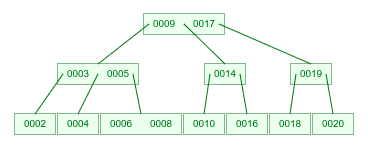
\includegraphics[]{graphics/b-trees/b-tree-example.png}
    
    \noindent Odmianą B-drzew są drzewa B+, które różnią się tym, że wszystkie wartości trzymane są w liściach oraz mają powiązania pomiędzy liśćmi (tak aby można było po kolei przejść wszystkie wartości w liściach).
    
    \subsection{Wyszukiwanie}
    Wyszukiwanie przebiega bardzo podobnie jak w drzewie BST, z tą różnicą, że nie mamy tylko lewego i prawego poddrzewa, a możemy mieć ich więcej, więc musimy zadecydować, do którego pójść.
    Oczywiście szukana wartość może również znajdować się na danym poziomie. Wtedy kończymy wyszukiwanie.
    Ponieważ rząd drzewa zazwyczaj jest wysoki (np. 1024), aby usprawnić wyszukiwanie zadanej wartości w danym węźle, najczęściej używamy wyszukiwania binarnego. \\
    
    \subsection{Wstawianie}
    Aby wstawić wartość wyszukujemy liść, do którego powinna trafić, a następnie wstawiamy ją w odpowiednie miejsce w tym liściu. \\
    \noindent Jeżeli jednak okazałoby się, że liść ma już za dużo kluczy (wartości) ($\geq K$), wtedy musimy go podzielić - jedną z wartości z liścia przenosimy w odpowiednie miejsce do rodzica, a jako prawego i lewego syna tej przeniesionej wartości wstawiamy odpowiednio liście powstałe po podzieleniu tego oryginalnego liścia. \\
    \noindent Jeżeli okazałoby się, że po przeniesieniu wartości z liścia do rodzica, rodzic ma za dużo kluczy (wartości), całą operację dzielenia powtarzamy rekurencyjnie na rodzicu - w razie potrzeby aż do korzenia. \\
    
    \subsection{Usuwanie}
    Usuwanie rozpoczynamy od znalezienia wartości, którą chcemy usunąć \\
    \noindent Następnie bierrzemy największą wartość z lewego podrzewa lub najmniejszą wartość z prawego poddrzewa i wstawiamy w miejsce usuwanego elementu \\
    \noindent Jeżeli w drzewie zostały naruszone warunki dotyczące ilości dozwolonych elementów w węźle, musimy to drzewo zrównoważyć. Proces ten jest generalnie dośc skomplikowany i ciężki do opisania algorytmem ze względu na mnogość możliwych przypadków, dlatego najlepiej spojrzeć na część praktyczną i przykłady.
    
    \newpage
    
    
    \section{Drzewa AVL: rotacje, operacje z wykorzystaniem rotacji i ich złożoność.}
    Drzewa AVL są odmianą drzew BST, w której dla każdego węzła mamy dodatkowy warunek: różnica między wysokością prawego i lewego poddrzewa danego węzła nie może byc większa niż 1.
    Spełnienie tego warunku zapewnia nam dobre zrównoważenie drzewa, a co za tym idzie utrzymanie szybkości operacji wywszukiwania w tym drzewie.\\
    
    \noindent Operacja wyszukiwania w drzewie AVL jest identyczna, jak dla zwykłego drzewa BST, natomiast w przypadku operacji wstawiania i usuwania, przebiegają one na początku tak samo jak w zwykłych BST, natomiast potem w razie potrzeby należy drzewo zrównoważyć poprzez rotacje. \\
    
    \noindent Operacje wyszukiwania, wstawiania oraz usuwania mają złożoność $O(\log_{2} n)$, gdzie n to ilość elementów w drzewie
    
    \subsection{Rotacje}
    \begin{multicols}{2}
    \textbf{Rotacja RR} \\
    
    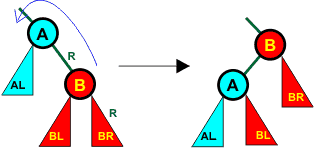
\includegraphics[width=0.8\linewidth]{graphics/avl-trees/rr-rotation.png}
    \columnbreak \\
    \textbf{Rotacja LL} \\
    
    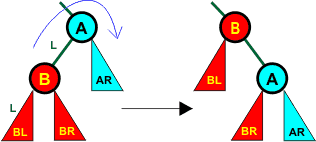
\includegraphics[width=0.8\linewidth]{graphics/avl-trees/ll-rotation.png}
    \end{multicols}
    
    \textbf{Rotacja RL} \\
    
    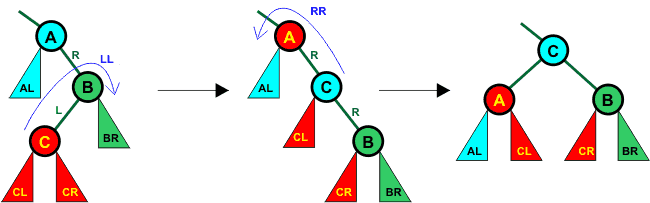
\includegraphics[width=\linewidth]{graphics/avl-trees/rl-rotation.png} \\

    \textbf{Rotacja LR} \\
    
    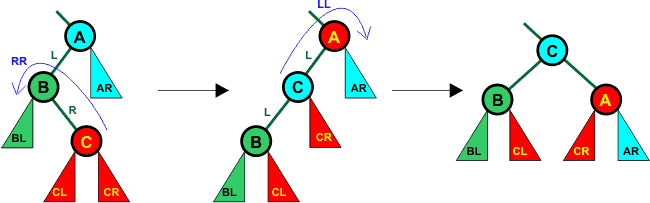
\includegraphics[width=\linewidth]{graphics/avl-trees/lr-rotation.png} \\
    
    \noindent Gdy \texttt{nierównowaga drzewa} idzie dwa razy na prawo (tzn. gdy dla danego węzła prawe poddrzewo jest głębsze niż lewe i potem dla pierwszego węzła prawego poddrzewa jego prawe poddrzewo jest głębsze) do zbalansowania używamy rotacji RR, natomiast, gdy nierównowaga idzie najpierw na prawo potem na lewo, używamy rotacji RL, itd.
    
    \section{Algorytmy przeszukiwania wszerz i w głąb w grafach.}
    \section{Algorytmy wyszukiwania najkrótszej ścieżki (Dijkstry oraz Bellmana-Forda).}
    \section{Programowanie dynamiczne: podział na podproblemy, porównanie z metodą "dziel i zwyciężaj".}
    \section{Algorytm zachłanny: przykład optymalnego i nieoptymalnego wykorzystania.}
    
    \newpage
    
    \section{Kolorowania wierzchołkowe (grafów planarnych) i krawędziowe grafów, algorytmy i ich złożoności.}
    
    \subsection{Kolorowanie krawędziowe grafów}
    Problem kolorowania krawędzi, podobnie jak klasycznego kolorowania wierzchołków, jest NP-trudny – nie istnieją wielomianowe algorytmy kolorujące grafy zawsze w sposób optymalny.
    \\\\
    Przykład nieopytymalnego algorytmu kolorowania krawędziowego:
    \begin{enumerate}
        \item Użyj BFS (Breadth First Search - Przeszukiwanie wszerz) do poruszania się po grafie.
        \item Wybierz wierzchołek i nadaj różne kolory jego krawędziom.
        \item Przejdź do kolejnego wierzchołka.
        \item Powtarzaj aż wszyskie krawędzie zostaną pokolorowane.
    \end{enumerate}
    
    \subsection{Kolorowanie wierzchołkowe grafów planarnych}
    
    \begin{definition}
        Graf planarny - graf, który można narysować na płaszczyźnie tak, by krzywe obrazujące krawędzie grafu nie przecinały się ze sobą.
    \end{definition}
    
    \begin{theorem}
        Liczba chromatyczna grafu planarnego jest równa lub mniejsza niż 4
    \end{theorem}
    
    Każdy graf planarny można pokolorować 5 kolorami w czasie liniowym.
    
    
    
    
    
    \newpage
    
    \section{Algorytmy wyszukiwania minimalnego drzewa rozpinającego: Boruvki, Prima i Kruskala.}
    
    \subsection{Algorytm Boruvki}
    \begin{enumerate}
        \item Zainicjalizuj każdy wierzchołek jako osobny zbiór.
        \item Znajdź krawędź z najmniejszą wagą łączącą ten zbiór z innym. Dodaj tą krawędź do MST.
        \item Powtarzaj krok 2 dla każdego zbioru dopóki istnieje więcej niż jeden zbiór.
    \end{enumerate}
    \textbf{Złożoność:} $O(ElogV)$.
    
    
    \subsection{Algorytm Prima}
    \begin{enumerate}
        \item Zainicjalizuj drzewo jednym wierzchołkiem, wybranym losowo z grafu.
        \item Powiększ drzewo o jeden wierzchołek z najmniejszą wagą który łączy drzewo z wierzchołkami jeszcze nieuwzględnionymi.
        \item Powtarzaj krok 2 aż wszystkie wierzchołki znajdą się w drzewie.
    \end{enumerate}
    \textbf{Złożoność:} Zależy od użytych struktur danych. $O(V^2)$ lub $O(ElogV)$ jeśli użyta została lista sąsiedztwa
    
    
     
    \subsection{Algorytm Kruskala}

    \begin{enumerate}
        \item Posortuj krawędzie niemalejąco pod względem wag.
        \item Wybierz krawędź o najmniejszej wadze. Sprawdź czy tworzy cykl z MST utworzonym do tej pory. Jeśli nie, uwzględnij tą krawędź w MST. W przeciwnym wypadku, odrzuć.
        \item Powtarzaj krok 2 aż otrzymasz $V-1$ krawędzi w MST
    \end{enumerate}
        
    \textbf{Złożoność:} Sortowanie krawędzi zajmuje $O(ElogE)$. Po sortowaniu, iterujemy po krawędziach i używamy algorytmu find-union który może zająć $O(logV)$. Zatem ogólna złozoność to $O(ElogE+ElogV)$. Wartość E jest mniejsza niż $V^2$, więc $O(logV)$ $=$ $O(logE)$. Złożoność: $O(ElogE)$ lub $O(ElogV)$. 

    \newpage

    \section{Najważniejsze algorytmy wyznaczania otoczki wypukłej zbioru punktów w układzie współrzędnych (Grahama, Jarvisa, algorytm przyrostowy (quickhull)).}

    \begin{definition}
        \textbf{Algorytm Grahama} - złożoność $O(n \log n)$.
        \begin{enumerate}
            \item Wybierz punkt (ozn. O) o najniższej wartości współrzędnej y.
            \item Przesuń wszystkie punkty tak, by punkt O pokrył się z początkiem układu współrzędnych.
            \item Posortuj punkty leksykograficznie względem:
            \begin{itemize}
                \item kąta pomiędzy wektorem $OP_i$ a dodatnią osią układu współrzędnych,
                \item odległości punktu $P_i$ od początku układu współrzędnych.
            \end{itemize}
            \item Wybierz punkt (ozn. S) o najmniejszej współrzędnej y; jeśli kilka punktów ma tę samą współrzędną
            y, wybierz spośród nich ten o najmniejszej współrzędnej x.
            \item Przeglądaj listę posortowanych punktów poczynając od punktu S:
            \begin{itemize}
                \item Od bieżącej pozycji weź trzy kolejne punkty (ozn. A, B, C).
                \item Jeśli punkt B leży na zewnątrz trójkąta AOC, to może należeć do otoczki wypukłej. Przejdź do następnego punktu na liście.
                \item Jeśli punkt B leży wewnątrz trójkąta AOC, to znaczy, że nie należy do otoczki. Usuń punkt B z listy i cofnij się o jedną pozycję (o ile bieżąca pozycja jest różna od początkowej).
            \end{itemize}
        \end{enumerate}
    \end{definition}

    \begin{definition}
        \textbf{Algorytm Jarvisa} - średnia złożoność $O(kn)$, gdzie n liczba punktów, k liczba punktów należących do otoczki; pesymistyczna - $O(n^2)$.
        \begin{enumerate}
            \item $P_1$ – punkt na otoczce wypukłej o najmniejszej współrzędnej y (jeśli jest więcej niż jeden, wybierany jest ten o najmniejszej współrzędnej x),
            \item $P_{0}:=[-\infty ,y(P_{1})]$,
            \item $i:=1$,
            \item powtarzaj:
            \begin{itemize}
                \item $P_{i+1}$ – punkt $N$, dla którego kąt $P_{i-1}P_{i}N$ jest największy,
                \item jeśli $N=P_{1}$, koniec iterowania,
                \item $:=i+1$,
            \end{itemize}
            \item ostatecznie otoczkę tworzą punkty $P_{1\dots i}$.
        \end{enumerate}

        Implementację można usprawnić, odrzucając w każdej iteracji punkty znajdujące się po prawej stronie wektora $P_{1}P_{i}$, ponieważ na pewno nie będą należały do otoczki. Zabieg ten nie wpływa jednak na asymptotyczną złożoność obliczeniową algorytmu.
    \end{definition}

    \begin{definition}
        \textbf{Quickhull} - średnia złożoność $O(n \log n)$, pesymistyczna złożoność - $O(n^2)$.

        Przygotowanie danych:
        \begin{enumerate}
            \item Znajdź w zbiorze punktów dwa skrajne punkty o minimalnej i maksymalnej współrzędnej x (A i B).
            \item Podziel zbiór punktów na dwa podzbiory $S_1$ i $S_2$ znajdujące się nad i pod prostą $AB$.
            \item Wywołaj rekurencyjnie QuickHull(A, B, $S_1$) i QuickHull(B, A, $S_2$).
        \end{enumerate}

        QuickHull(A, B, P):
        \begin{enumerate}
            \item Jeśli $P$ jest pusty – koniec.
            \item Jeśli $P$ ma jeden element, ten punkt należy do otoczki – koniec.
            \item W przeciwnym razie:
            \begin{itemize}
                \item Znajdź w $P$ punkt $C$ najbardziej oddalony od prostej $AB$. Ten punkt należy do otoczki wypukłej.
                \item Odrzuć wszystkie punkty z wnętrza trójkąta $ABC$, nie mogą należeć do otoczki.
                \item Znajdź zbiór $S_1$ punktów znajdujących się po prawej stronie prostej $AC$C oraz analogiczny
                zbiór $S_2$ dla prostej $BC$. (Stronę określa znak równania ogólnego prostej).
                \item Wywołaj rekurencyjnie QuickHull(A, C, $S_1$) i QuickHull(B, C, $S_2$).
            \end{itemize}
        \end{enumerate}
    \end{definition}

    \newpage

    \section{Problemy P, NP, NP-zupełne i zależności między nimi. Hipoteza P vs. NP.}
    \begin{definition}
        \textbf{Problem P} (ang. \textit{deterministic polynomial}, deterministycznie wielomianowy) – problem decyzyjny,
        dla którego rozwiązanie można \textbf{znaleźć} w czasie wielomianowym.
    \end{definition}

    \begin{definition}
        \textbf{Problem NP} (ang. \textit{nondeterministic polynomial}, niedeterministycznie wielomianowy) – problem
        decyzyjny, dla którego rozwiązanie można \textbf{zweryfikować} w czasie wielomianowym.
    \end{definition}

    \begin{theorem}
        $\mathbf{P \stackrel{?}{=} NP}$. Każdy problem P jest NP, jednak nie wiadomo czy istnieje problem NP niebędący P.
    \end{theorem}

    \begin{definition}
        \textbf{Problem NP-zupełny} (ang. \textit{NP-Complete}) – problem, który \textbf{należy do klasy NP} oraz dowolny
        problem należący do NP może być do niego \textbf{zredukowany w czasie wielomianowym}. Czasami zamiast redukcji w
        czasie wielomianowym używa się redukcji w pamięci logarytmicznej. Taka definicja problemów NP-zupełnych
        implikuje fakt, że jeśli tylko potrafimy rozwiązać jakikolwiek problem NP-zupełny w czasie wielomianowym,
        to potrafimy rozwiązać w takim czasie wszystkie problemy NP.\\

        Pierwszym problemem którego NP-zupełność wykazano był problem SAT, czyli problem spełnialności formuł zdaniowych.
    \end{definition}

    \newpage

    \section{Automat minimalny, wybrany algorytm minimalizacji.}
    \subsection{Automat minimalny}
    \begin{definition}
    Automat $\mathcal{A} = (S, A, f, s_{0}, T)$ rozpoznający język L nazywamy automatem minimalnym, jeśli posiada najmniejszą liczbę stanów spośród wszystkich automatów rozpoznających język L
    \end{definition}
    
    \begin{definition}
    Dla dowolnego języka $L \in \mathcal{REC}(A^{*})$ automat
		\begin{center}
			$\mathcal{A}_{P_{L}^{r}} = (A^{*} / P_{L}^{r}, A, f^{*}, [1]_{P_{L}^{r}}, T)$,
		\end{center}
	gdzie $T = \{[w]_{P_{L}^{r}} : w \in L \}$ jest automatem minimalnym rozpoznającym język L
    \end{definition}
    \begin{definition}
    \textbf{Konstrukcja automatu minimalnego z wykorzystaniem prawej kongruencji automatowej} \\
	$L \subset A^{*}$ - dowolny język \\
	$\Theta_{L} \subset A^* \times A^*$ - relacja równoważności dzieląca $A^*$ na dwie klasy:
	\begin{center}
		L i $A^*$ \ L
    \end{center}
    $\rho_i$ dla $i \in \mathbb{N}$ - zstępujący ciąg relacji: \\
    $\rho_1 = \Theta_L$, \\
    $\rho_i = \{(u, w) \in A^* \times A^* : \forall a \in A \cup \{\textbf{1}\} (ua, wa) \in \rho_{i-1} \}$ dla i = 2, ... \\
    Wtedy
    \begin{center}
		$\bigcap\limits_{i \in \mathbb{N}} \rho_i = P^r_L$
	\end{center}
    \end{definition}
    
    
    \subsection{Minimalizacja automatu}
    \begin{definition}
    		\textbf{Algorytm ``Minimalizuj 1''} \\
    		\url{http://wazniak.mimuw.edu.pl/index.php?title=J\%C4\%99zyki\%2C_automaty_i_obliczenia/Wyk\%C5\%82ad_5:_Algorytmy_konstrukcji_automatu_minimalnego} \\
		Wejście L - język \\
        	Wyjście: automat minimalny $\mathcal{A} = (S_L, A, f_F, s_L, T_L)$ taki, że $L\mathcal{A} = L$
        	\begin{lstlisting}
$S_L \leftarrow \{L\};$
Put$(\mathcal{L}, L);$
while $\mathcal{L} \neq \emptyset$ do
  M $\leftarrow$ \textbf{zdejmij} $(\mathcal{L})$;
  foreach $a \in A$ do
    N $\leftarrow a^{-1}M$;
    if $N \cap S_L = \emptyset$ then
      $S_L \leftarrow S_L \cup \{N\}$;
      Put$(\mathcal{L}, N);$
    end if
  end for
end while
foreach $M \in S_L$ do
  foreach $a \in A$ do
    $f_L(M, a) \leftarrow a^{-1}M$;
  end for
end for
$s_L \leftarrow L$;
$T_L \leftarrow \{u^{-1}L : u \in L\}$;
return $\mathcal{A}'$;
	    	\end{lstlisting}
    \end{definition}
    
    \section{Lemat o pompowaniu dla języków regularnych.}
    \begin{definition}
    Niech $L \subset A^*$ będzie językiem rozpoznawalnym. Istnieje liczba naturalna $N \geq 1$ taka, że dowolne słowo $w \in L$ o długości $|w| \geq N$ można rozłożyć na katenację:
    \begin{center}
    $w = v_1uv_2$
    \end{center}
    gdzie $v_1, v_2 \in A^*, u \in A^+, |v_1u| < N$ oraz
    \begin{center}
    $v_1u^*v_2 \subset L$
    \end{center}
    \end{definition}
    
    \begin{definition}
    Jeśli rozpoznawalny język $L \subset A^*$ jest nieskończony, to istnieją
    $v_1, v_2 \in A^*, u \in A^+$, takie, że
    \begin{center}
	$v_1u*v_2 \subset L$
    \end{center}
    \end{definition}
    
    
    
    \section{Warunki równoważne definicji języka regularnego: automat, prawa kongruencja syntaktyczna, wyrażenia regularne.}
    \section{Automaty niedeterministyczne i deterministyczne (w tym ze stosem); determinizacja.}
    \section{Problemy rozstrzygalne i nierozstrzygalne w teorii języków.}
    \section{Klasy języków w hierarchii Chomsky’ego oraz ich zamkniętość ze względu na operacje boolowskie, homomorfizmy, itp.}


    {\Large Wytwarzanie oprogramowania}

    \section{Reprezentacja liczb całkowitych; arytmetyka.}
    \section{Reprezentacja liczb rzeczywistych; arytmetyka zmiennopozycyjna.}

    \newpage

    \section{Różnice w wywołaniu funkcji statycznych, niestatycznych i wirtualnych w C++.}

    \subsection{Funkcje statyczne.}
    \begin{itemize}
        \item \textbf{Globalne funkcje statyczne} to funkcje o zakresie widoczności ograniczonym do pliku źródłowego, który je
        zawiera (a dokładniej do ich \textit{jednostce translacji}, czyli pliku który jest kompilowany - zatem pliku
        źródłowego wraz z dołączonymi includami).
        \item \textbf{Metody statyczne klas} to metody których wywołanie jest niezależne od instancjonowania klasy -
        wszystkie instancje klasy współdzielą kopię statycznych metod i pól. Instancja klasy nie jest nam potrzebna
        do wywołania statycznej metody (aczkolwiek można jej użyć).
    \end{itemize}

    \begin{minted}{cpp}
        #include <iostream>
        using namespace std;

        // statyczna funkcja globalna dostępna tylko z naszego pliku
        static void sayHello(){
            cout << "hello" << endl;
        }

        class ExampleClass {
            public:
                static void sayBye(){
                    cout  << "bye" << endl;
                }
        };

        int main(){
            sayHello();

            ExampleClass::sayBye(); // wywołanie bez instancjonowania klasy

            ExampleClass e();
            e.sayBye(); // wywołanie dla instancji klasy
        }
    \end{minted}

    \subsection{Funkcje niestatyczne.}
    \begin{itemize}
        \item \textbf{Niestatyczne funkcje globalne} są dostępne ze wszystkich plików, które includują zawierające
        je plik źródłowy - trzeba zatem uważać na konflikty nazw.
        \item \textbf{Nietstatyczne metody klas} wymagają do wywołania instancji klasy - mogą zachowywać się różnie
        dla różnych instancji; mogą być oznaczone \texttt{final} i \texttt{override}.
    \end{itemize}

    \begin{minted}{cpp}
        #include <iostream>
        using namespace std;

        // niestatyczna funkcja globalna dostępna dla wszystkich plików
        void sayHello(){
            cout << "hello" << endl;
        }

        class ExampleClass {
        public:
            void sayBye(){
                cout  << "bye" << endl;
            }
        };

        int main(){
            sayHello();

            // ExampleClass::sayBye() -  wywołanie niepoprawne

            ExampleClass e();
            e.sayBye(); // wywołanie dla instancji klasy
        }
    \end{minted}

    \subsection{Funkcje wirtualne.}
    \begin{itemize}
        \item \textbf{Wirtualne metody klas} są przydatne polimorfiźmie.
        \item W przypadku zwykłej metody, wywołanie jej dla wskaźnika typu klasy podstawowej zawsze wywoła instancję
        z klasy podstawowej, nawet jeżeli wskaźnik będzie tak naprawdę wskazywał na klasę pochodną.
        \item Słowo kluczowe \texttt{virtual} wymusza dedukcję której metody użyć na podstawie zawartości wskaźnika,
        a nie jego typu. Dedukcja następuje w czasie wykonania programu.
    \end{itemize}

    Bez \texttt{virtual}:
    \begin{minted}{cpp}
        #include <iostream>
        using namespace std;

        struct Base {
            void f() {
            cout << "base" << endl;
            }
        };

        struct Derived : Base {
            void f() {
            cout << "derived" << endl;
            }
        };

        int main(){
        Base b;
        Derived d;

        // call through reference
        Base& br = b; // the type of br is Base&
        Base& dr = d; // the type of dr is Base& as  well
        br.f(); // "base"
        dr.f(); // "base"

        // cal through pointer
        Base* bp = &b; // the type of bp is Base*
        Base* dp = &d; // the type of dp is Base* as  well
        bp->f(); // "base"
        dp->f(); // "base"

        return 0;
        }
    \end{minted}


    Przy użyciu \texttt{virtual}:
    \begin{minted}{cpp}
    #include <iostream>
    using namespace std;

    struct Base {
        virtual void f() {
        cout << "base" << endl;
        }
    };

    struct Derived : Base {
        void f() override { // 'override' is optional
        cout << "derived" << endl;
        }
    };

    int main(){
        Base b;
        Derived d;

        // call through reference
        Base& br = b; // the type of br is Base&
        Base& dr = d; // the type of dr is Base& as  well
        br.f(); // "base"
        dr.f(); // "derived"

        // call through pointer
        Base* bp = &b; // the type of bp is Base*
        Base* dp = &d; // the type of dp is Base* as  well
        bp->f(); // "base"
        dp->f(); // "derived"

        return 0;
    }
    \end{minted}

    \newpage

    \section{Sposoby przekazywania parametrów do funkcji (przez wartość, przez referencję). Zalety i wady.}

    \subsection{Przekazywanie przez wartość.}

    Przekazywanie argumentu przez wartość oznacza, że argumentem może być \textbf{rvalue} (np. wyrażenie arytmetyczne), a przekazanie
    lvalue (zmiennej) powoduje utworzenie \textbf{kopii}.
    \begin{itemize}
        \item Za zaletę można uznać fakt możliwości użycia wyrażenia w wywołaniu (zakładając że nie używamy wyniku tego
        wyrażenia nigdzie indziej - nie potrzebujemy tworzyć zbędnej zmiennej).
        \item Kwestia tworzenia kopii może być zaletą lub wadą - umożliwia nam to swobodne modyfikowanie wartości
        bez modyfikowania oryginalnej zmiennej (co może być chcianą funkcjonalnością), ale może stanowić niepotrzebne obciążenie
        w przypadku gdy dana zmienna nie jest lub może być modyfikowana (wtedy tworzenie kopii jest niepotrzebne).
    \end{itemize}

    \begin{minted}{cpp}
        #include <iostream>
        using namespace std;

        void add2(int x){
            x += 2;
            cout << x << endl; // 7
        }

        int main(){
            int a = 5;
            cout << a << endl; // 5

            add2(a);
            cout << a << endl; // 5

            return 0;
        }
    \end{minted}

    \subsection{Przekazywanie przez referencję.}
    Funkcja otrzymuje jako argument adres zmiennej, a nie jej wartość. Mając adres może odwołać się do pamięci tej
    zmiennej i zmienić jej zawartość. Wszelka modyfikacja takiego argumentu wewnątrz funkcji powoduje zmianę skojarzonej
    z tym argumentem zmiennej.
    \begin{itemize}
        \item Zaletą jest nietworzenie niepotrzebnych kopii, możliwość zmiany zmiennej spoza zakresu funkcji (zamiast
        np. zwracania i przypisywania nowej wartości).
        \item Nieprzemyślane użycie może spowodować nieprzewidzianą przez programistę zmianę zawartości zmiennej.
        \item Brak możliwości użyca wyrażenia jako argumentu funkcji - musimy zapisać jego wynik w zmiennej, by móc
        ją przekazać.
    \end{itemize}

    \begin{minted}{cpp}
        #include <iostream>
        using namespace std;

        void add2(int & x){
            x += 2;
            cout << x << endl; // 7
        }

        int main(){
            int a = 5;
            cout << a << endl; // 5

            add2(a);
            cout << a << endl; // 7

            return 0;
        }
    \end{minted}

    \newpage

    \section{Wskaźniki, arytmetyka wskaźników, różnica między wskaźnikiem a referencją w C++.}
    \begin{definition}
    	\textbf{Wskaźnik} – typ zmiennej odpowiedzialnej za przechowywanie adresu do innej zmiennej (innego miejsca w pamięci) w obrębie naszej aplikacji.
    	Wskaźnik może wskazywać na jakąś zmienną, strukturę, tablicę czy nawet funkcję.
    \end{definition}
    
    \begin{definition}
    	\textbf{Operatory związane ze wskaźnikami w C++}
    	\begin{minted}{cpp}
int a = 5;

// Creation of pointer to int variable
int *intPtr = nullptr;  // In older versions NULL

// Using & (ampersand) to get address of variable
// then assign to pointer
intPtr = &a;

// Using * as dereference operator
// to get value of pointed variable
cout << *intPtr << endl;
    	\end{minted}
    \end{definition}
    
    \begin{definition}
    	\textbf{Arytmetyka wskaźników} \\
    	Mając wskaźnik \texttt{int *p} wskazujący na hipotetyczny adres 10, wykonując na nim operację \texttt{p+2} dostajemy wskaźnik wskazujący na adres \texttt{10 + 2*sizeof(int)}
    	czyli zakładając, że typ \texttt{int} zajmuje w naszym kompilatorze 4 bajty dostajemy \texttt{10 + 2*4} = \texttt{18}. \\
    	Jest to przydatne szczególnie przy operowaniu na strukturach, których pola są ułożone po kolei w pamięci, np. tablice:
    	\begin{minted}{cpp}
int *a = new int[10] {0, 10, 20, 30, 40, 50, 60, 70, 80, 90};
// Now a pointing to first element in array
cout << *a << endl;  // 0

// Using dereference operator with pointer arithmetic
cout << *(a+3) << endl;  // 30
    	\end{minted}
    	Jak więc widać \texttt{*(a+i)} $\Leftrightarrow$ \texttt{a[i]}.
    \end{definition}
    
    \begin{definition}
    \textbf{Wskaźnik a referencja} \\
    Referencję możemy traktować jako dodatkową nazwę na juz istniejący obiekt. Jest to coś w rodzaju stałego wskaźnika.
    Składnia referencji zabrania jednak wykonywania operacji znanych dla wskaźników:
    \begin{itemize}
        \item Dla referencji nie można zmienić referowanego obiektu - raz ustawiony (a musi być ustawiony prawie zawsze podczas jej deklaracji) nie zmienia się przez cały czas jej życia
        \item Nie jest dostępna arytmetyka referencji (w przeciwieństwie do arytmetyki wskaźników)
    \end{itemize}
    Po kompilacji (w kodzie maszynowym) referencje i wskaźniki niczym się nie różnią.
    Korzystając z referencji świadomie rezygnujemy z pewnych możliwości oferowanych nam przez wskaźniki. W zamian dostajemy:
    \begin{itemize}
	\item Łatwiejszą notację - nie musimy używać operatora wyłuskania (\texttt{*}) do odwoływania się do obiektu
	\item Większe bezpieczeństwo - brak arytmetyki dla referencji znacznie utrudnia popełnienie błędów związanych z niepoprawnym odwołaniem do pamięci
    \end{itemize}
    \end{definition}
    
    \noindent \textbf{Przykład użycia referencji}
    \begin{minted}{cpp}
int n = 6;

// Deklaracja referencji na typ int i przypisanie referowanego obiektu
// Referencję deklarujemy dodając & (ampersand) między nazwą typu a zmiennej
// (nie mylić z & jako operatorem pobrania adresu omawianym przy wskaźnikach)
int &r = n;

cout << r << endl; // 6

// Zmiana wartości odwołując się do referncji
// zmienia tak na prawdę wartość oryginalnego obiektu
r = 7;

cout << n << endl; //7
    \end{minted}    
    
    \newpage
    
    \section{Podstawowe założenia paradygmatu obiektowego: dziedziczenie, abstrakcja, enkapsulacja, polimorfizm.}
    \begin{definition}
	\textbf{Dziedziczenie (kompozycja)} \\
    	Umożliwia stworzenie hierarchii obiektów w programie. Polega na przejęciu właściwości i funkcjonalności obiektów innej klasy
    	i ewentualnej modyfikacji tych właściwości i funkcjonalności w taki sposób, by były one bardziej wyspecjalizowane.
    	\begin{minted}{cpp}
class Mammal {
public:
  void feed() {
    cout << "sucking" << endl;
  }
		
  virtual void giveVoice() = 0; // Pure virtual method
};

class Cat : public Mammal {
public:
  void giveVoice() override {
    cout << "meow" << endl;
  }
};

int main() {
  Cat cat = new Cat();
  cat.feed();
  cat.giveVoice();
  /*
  sucking
  meow
  */
}
    	\end{minted}
    \end{definition}
    
    \begin{definition}
    \textbf{Abstrakcja} \\
    Każdy obiekt w systemie służy jako model abstrakcyjnego "wykonawcy", który może wykonywać pracę, opisywać i zmieniać swój stan, oraz komunikować się
    z innymi obiektami w systemie, bez ujawniania, w jaki sposób zaimplementowano dane cechy.
    \begin{minted}{cpp}
class DiscountComputator {
private:
  int factor;
  ...

public:  
  // Setter
  void setFactor(int factor) {
    this.factor = factor;
  }
  
  double compute(double price) {
    ...
  }
};

int main() {
  DiscountComputator dc = new DiscountComputator();
  
  dc.setFactor(5);
  
  // We are not interested how it is calculated
  double result = dc.compute(123.45);
}
    \end{minted}
    \end{definition}
    
    \begin{definition}
    \textbf{Enkapsulacja} \\
    Enkapsulacja zapewnia, że obiekt nie może zmieniać stanu innych obiektów w nieokreślony sposób.
    Każdy typ obiektu dostarcza interfejsu, który określa sposób współpracy z innymi obiektami.
    Jedynie za pomocą określonych metod mamy możliwość zmienić stan obiektu, bezpośredni dostęp
    do zmiennych jest zabroniony.
    \begin{minted}{cpp}
class MyClass {
private:
  int field;
  
public:
  // Setter
  void setField(int field) {
    this.field = field;
  }
  
  // Getter
  int getField() {
    return field;
  }
};

int main() {
  MyClass clazz = new MyClass();
  
  clazz.setField(5);
  int field = clazz.getField();
  
  /*
  // The `field` is private, so the following
  // will cause an error during compilation
  clazz.field = 5;
  int field = clazz.field;
  */
}
    \end{minted}
    \end{definition}
    
    \begin{definition}
    \textbf{Polimorfizm} \\
    Referencje i wskaźniki obiektów mogą dotyczyć obiektów różnego typu, a wywołanie metody dla referencji spowoduje zachowanie
    odpowiednie dla pełnego typu obiektu wywoływanego. Zazwyczaj można wyróżnić dwa rodzaje polimorfizmu: dynamiczne - wykonywane podczas działania programu,
    a także statyczne - na etapie kompilacji.
    \begin{minted}{cpp}
class Point {
protected:
    int x, y;
public:
    // Constructor with initializer list
    Point(int x, int y) : x(x), y(y) {
    }

    virtual void printPoint() {
        cout << "(" << x << ", " << y << ")" << endl;
    }

    void printClassName() {
        cout << "Point" << endl;
    }
};

class ColoredPoint : public Point {
protected:
    int color;
public:
    // Constructor with initializer list
    ColoredPoint(int x, int y, int color)
        : Point(x, y), color(color) {
    }

    void printPoint() {
        cout << "(" << x << ", " << y
            << ", color = " << color << ")" << endl;
    }

    void printClassName() {
        cout << "ColoredPoint" << endl;
    };
};
	\end{minted}
	\end{definition}
	\begin{definition} \textbf{} \\
	\begin{minted}{cpp}
int main() {
    Point *p = new ColoredPoint(1, 2, 3);
    p->printPoint();
    p->printClassName();
    delete p;

    ColoredPoint *cp = new ColoredPoint(1, 2, 3);
    cp->printPoint();
    cp->printClassName();
    delete cp;

    return 0;
}

/* Output:
   (1, 2, color = 3)
   Point
   (1, 2, color = 3)
   ColoredPoint
*/
    \end{minted}
    
    Jak widzimy dla obu wskaźników instancjonujemy klasę \texttt{ColoredPoint}. W przypadku wskaźnika \texttt{p} i wywołania metody \texttt{printClassName}
    została wywołana meteda z klasy \texttt{Point}, mimo że wskaźnik wskazuje na obiekt typu \texttt{ColoredPoint}. Dzieje się tak, ponieważ kompilator domyślnie
    bierzez pod uwagę typ wskaźnika, a nie wskazywanego obiektu. Aby temu zaradzić musimy oznaczyć wołaną metodę jako \texttt{virtual}. Spowoduje to, że
    kompilator przy wywołaniu tej metody weźmie pod uwagę typ wskazywanego obiektu, a nie typ wskaźnika, czego przykładem jest metoda \texttt{printPoint}
    z powyższego kodu.
    \end{definition}
    
    \newpage
    
    \section{Funkcje zaprzyjaźnione i ich związek z przeładowaniem operatorów w C++.}
    \section{Programowanie generyczne na podstawie szablonów w języku C++.}
    \section{Podstawowe kontenery w STL z szerszym omówieniem jednego z nich.}
    \section{Obsługa sytuacji wyjątkowych w C++.}
    \section{Obsługa plików w języku C.}
    \section{Model wodospadu a model spiralny wytwarzania oprogramowania.}
    \section{Diagram sekwencji i diagram przypadków użycia w języku UML.}
    \section{Klasyfikacja testów.}
    \section{Model Scrum: struktura zespołu, proces wytwarzania oprogramowania, korzyści modelu.}
    \section{Wymagania w projekcie informatycznym: klasyfikacja, źródła, specyfikacja, analiza.}
    \section{Analiza obiektowa: modele obiektowe i dynamiczne, obiekty encjowe, brzegowe i sterujące.}
    \section{Wzorce architektury systemów.}

    {\Large Inżynieria systemów}

    \section{Relacyjny model danych, normalizacja relacji (w szczególności algorytm doprowadzenia relacji do postaci Boyce’a-Codda), przykłady.}
    \section{Indeksowanie w bazach danych: drzewa B+, tablice o organizacji indeksowej, indeksy haszowe, mapy binarne.}
    \section{Podstawowe cechy transakcji (ACID). Metody sterowania współbieżnością transakcji, poziomy izolacji transakcji, przykłady.}
    \section{Złączenia, grupowanie, podzapytania w języku SQL.}
    \section{Szeregowalność harmonogramów w bazach danych.}
    \section{Definicja cyfrowego układu kombinacyjnego - przykłady układów kombinacyjnych i ich implementacje.}
    \section{Definicja cyfrowego układu sekwencyjnego - przykłady układów sekwencyjnych i ich implementacje.}
    \section{Minimalizacja funkcji logicznych.}
    \section{Programowalne układy logiczne PLD (ROM, PAL, PLA).}
    \section{Schemat blokowy komputera (maszyna von Neumanna).}
    \section{Zarządzanie procesami: stany procesu, algorytmy szeregowania z wywłaszczaniem.}
    \section{Muteks, semafor, monitor jako narzędzia synchronizacji procesów.}
    \section{Pamięć wirtualna i mechanizm stronicowania.}
    \section{Systemy plikowe - organizacja fizyczna i logiczna (na przykładzie wybranego systemu uniksopodobnego).}
    \section{Model ISO OSI. Przykłady protokołów w poszczególnych warstwach.}
    \section{Adresowanie w protokołach IPv4 i IPv6.}
    \section{Najważniejsze procesy zachodzące w sieci komputerowej od momentu wpisania adresu strony WWW do wyświetlenia strony w przeglądarce (komunikat HTTP, segment TCP, system DNS, pakiet IP, ARP, ramka).}
    \section{Działanie przełączników Ethernet, sieci VLAN, protokół STP.}
    \section{Rola routerów i podstawowe protokoły routingu (RIP, OSPF).}
    \section{Szyfrowanie z kluczem publicznym, podpis cyfrowy, certyfikaty.}
    \section{Wirtualne sieci prywatne, protokół IPsec.}


\end{document}
